% !TEX spellcheck = en-US
\chapter{Estimating Position and Orientation}
\label{cha:orientationEstimation} 
In this chapter we will focus on position and orientation estimation using the models~\eqref{eq:models-ssPose} and~\eqref{eq:models-ssOri} derived in \Chapterref{cha:models}. In \Sectionref{sec:oriEst-smoothingOpt}, we will first describe a method to solve the smoothing problem~\eqref{eq:models-smoothingProbs}. Subsequently, in \Sectionref{sec:oriEst-filteringOpt}--\Sectionref{sec:oriEst-compl}, we will derive different methods for solving the filtering problem~\eqref{eq:models-filteringProbs}. In each section, after a general introduction of the estimation method, we will illustrate the method by explicitly deriving algorithms to estimate the orientation using the state space model~\eqref{eq:models-ssOri}. The orientation estimation problem also illustrates the most important parts of the pose estimation problem, since most complexities lie in the parametrization of the orientation and in the nonlinear nature of  the orientation. In \Sectionref{sec:oriEst-orientationEstimation}, we show some characteristics of the different algorithms for the orientation estimation problem. In \Sectionref{sec:oriEst-poseEstimation}, we will discuss how the algorithms for orientation estimation can be extended to also estimate the position. Throughout this section, we assume that the sensors are calibrated, \ie we assume that we do not have any unknown parameters $\theta$ in our models. Because of this, the models that we use are the most basic models that can be used for position and orientation estimation using inertial sensors. 

\section{Smoothing in an optimization framework}
\label{sec:oriEst-smoothingOpt}
Perhaps the most intuitive way to solve the smoothing problem is by posing it as an optimization problem, where a \emph{\gls{map}} estimate is obtained as
\begin{align}
\hat{x}_{1:N} &= \argmax_{x_{1:N}} p(x_{1:N} \mid y_{1:N} ) \label{eq:oriEst-optLik} \nonumber \\
&= \argmax_{x_{1:N}} p(x_1) \prod_{t = 2}^N p(x_{t} \mid x_{t-1} ) p(y_t \mid x_t ). 
\end{align}
Here, we use the notation in terms of probability distributions as introduced in \Sectionref{sec:models-probModeling} and model the measurements and the state dynamics as described in~\Sectionref{sec:models-measModels} and~\Sectionref{sec:models-stateDynamics}, respectively. Furthermore, we assume that a prior on the initial state is obtained using the measurements at $t = 1$ as described in \Sectionref{sec:models-prior}. Because of this, the measurement model $p(y_1 \mid x_1)$ from~\eqref{eq:models-smoothingProbs} is explicitly omitted in~\eqref{eq:oriEst-optLik}. Note that in practice, we typically minimize $-\log p(x_{1:N} \mid y_{1:N})$ instead of maximizing $p(x_{1:N} \mid y_{1:N})$ itself, resulting in the optimization problem
\begin{align}
\argmin_{x_{1:N}} - \log p(x_1) - \sum_{t = 2}^N \log p(x_{t} \mid x_{t-1} ) - \sum_{t = 2}^N \log p(y_t \mid x_t ).\label{eq:oriEst-optNegLogLik}
\end{align}

There are various ways to solve problems of this kind, for instance particle smoothers \citep{lindstenS:2013}, an extended \gls{rts} smoother \citep{sarkka:2013} and optimization methods, see \eg \cite{nocedalW:2006,mattingleyB:2010}. The latter approach is closely related to iterated Kalman smoothers~\citep{bell:1994,jazwinski:1970}. We will solve the problem using an optimization method. Compared to extended \gls{rts} smoothers, optimization methods allow for more flexibility in the models that are being used. For instance, additional information outside of the standard state space model can straightforwardly be included. Optimization approaches are typically computationally heavier than extended \gls{rts} smoothers but less heavy than particle smoothers. The latter are capable of capturing the whole distribution, which is a clear advantage when the distributions are multi-modal. Optimization instead gives a point estimate and an associated measure of uncertainty. This is typically sufficient for position and orientation estimation using inertial sensors.

\subsection{Gauss-Newton optimization}
\label{sec:oriEst-GNopt}
To obtain a smoothing estimate of the position and orientation using optimization, we first recognize that for our models~\eqref{eq:models-ssPose} and~\eqref{eq:models-ssOri}, all probability distributions in~\eqref{eq:oriEst-optNegLogLik} are Gaussian. Let us therefore consider a slightly more general problem where the objective function consists of the product of Gaussian probability functions $p(e_i(x_{1:N}))$, $i = 1, \hdots, M$. Hence, the optimization problem can be written as
\begin{align}
\hat{x}_{1:N} = \argmin_{x_{1:N}} - \sum_{i = 1}^M \log p \left(e_i (x_{1:N}) \right). \label{eq:oriEst-optNegLogLikGaussian}
\end{align}
The probability distribution of $e_i(x)$ is given by
\begin{align}
p \left(e_i(x_{1:N}) \right) = \tfrac{1}{\sqrt{ (2 \pi)^{n_e} \det \Sigma_i}} \exp \left( - \tfrac{1}{2} e_i^\Transp(x_{1:N}) \Sigma_i^{-1} e_i(x_{1:N}) \right).
\end{align}
Omitting the terms independent of $x_{1:N}$, the optimization problem~\eqref{eq:oriEst-optNegLogLikGaussian} reduces to
\begin{align}
\label{eq:oriEst-generalNLS}
\hat x_{1:N} = \argmin_{x_{1:N}} \tfrac{1}{2} \sum_{i = 1}^M \| e_i(x_{1:N}) \|_{\Sigma_i^{-1}}^2, 
\end{align}
with $\| e_i(x_{1:N}) \|_{\Sigma_i^{-1}}^2 = e^\Transp_i(x_{1:N}) \Sigma_i^{-1} e_i(x_{1:N})$. The function that is being minimized in optimization problems, is often referred to as the \emph{objective function}.

The solution to~\eqref{eq:oriEst-generalNLS} can be found by studying the shape of the objective function as a function of $x_{1:N}$. This can be characterized in terms of the \textit{gradient} $\mathcal{G}(x_{1:N})$ and \textit{Hessian} $\mathcal{H}(x_{1:N})$, which provide information about the slope and curvature of the function, respectively. Defining 
\begin{align*}
e^\Transp_i(x_{1:N}) \Sigma_i^{-1} e_i(x_{1:N}) = \varepsilon_i^\Transp \varepsilon_i, \qquad \varepsilon_i = \Sigma_i^{-1/2} e_i(x_{1:N}),
\end{align*}
and the stacked variables 
\begin{align*}
\varepsilon = \begin{pmatrix} \varepsilon_1^\Transp & \cdots & \varepsilon^\Transp_M \end{pmatrix}^\Transp,
\end{align*}
the gradient and the Hessian are given by
\begin{subequations}
\label{eq:oriEst-gradHess}
\begin{align}
\mathcal{G}(x_{1:N}) &= \sum_{i = 1}^{M} \left( \tfrac{\diff \varepsilon_i}{\diff x_{1:N}} \right)^\Transp \varepsilon_i= \mathcal{J}^\Transp(x_{1:N}) \varepsilon, \label{eq:oriEst-gradient} \\
\mathcal{H}(x_{1:N}) &= \sum_{i = 1}^{M} \left( \left( \tfrac{\diff \varepsilon_i}{\diff x_{1:N}} \right)^\Transp \tfrac{\diff \varepsilon_i}{\diff x_{1:N}} + \varepsilon_i^\Transp \tfrac{\diff^2 \varepsilon_i}{\diff x_{1:N}^2} \right) \nonumber \\
&= \mathcal{J}^\Transp(x_{1:N}) \mathcal{J}(x_{1:N}) + \sum_{i = 1}^{M} \varepsilon_i^\Transp \tfrac{\diff^2 \varepsilon_i}{\diff x_{1:N}^2}. \label{eq:oriEst-hessian}
\end{align}
\end{subequations}
Note that for notational convenience, we have omitted the explicit dependence of~$\varepsilon$ on $x_{1:N}$. In~\eqref{eq:oriEst-gradHess}, we introduced the notation $\mathcal{J}(x_{1:N})$, which is the \emph{Jacobian} of the vector $\varepsilon$ with respect to $x_{1:N}$ as
\begin{align}
\mathcal{J}(x_{1:N}) = \begin{pmatrix} \tfrac{\diff \varepsilon_1}{\diff x_1} & \hdots & \tfrac{\diff \varepsilon_1}{\diff x_N} \\
\vdots & & \vdots \\
\tfrac{\diff \varepsilon_{M n_\varepsilon}}{\diff x_1} & \hdots & \tfrac{\diff \varepsilon_{ M n_\varepsilon}}{\diff x_N}
\end{pmatrix},
\end{align}
where $n_\varepsilon$ is the length of the vector $\varepsilon_i$. Instead of computing the true Hessian~\eqref{eq:oriEst-hessian}, we compute an approximation of it \citep{nocedalW:2006}, given by
\begin{align}
\label{eq:oriEst-approxHessian}
\mathcal{\hat{H}}(x_{1:N}) = \mathcal{J}^\Transp(x_{1:N}) \mathcal{J}(x_{1:N}).
\end{align}
This has the benefit of not having to compute second derivatives, at the same time as it guarantees that the Hessian is positive semidefinite. The downside of using~\eqref{eq:oriEst-approxHessian} is that it introduces an approximation.

The gradient and the (approximate) Hessian can be used to find the minimum of the objective function. For our models~\eqref{eq:models-ssPose} and~\eqref{eq:models-ssOri}, in which the functions $e_i(x_{1:N})$ are nonlinear, an estimate $\hat{x}_{1:N}$ can iteratively be computed as
\begin{align}
\label{eq:oriEst-GNiteration}
\hat x_{1:N}^{(k+1)} = \hat x_{1:N}^{(k)} - \beta^{(k)} \left( \mathcal{\hat{H}}(\hat x_{1:N}^{(k)}) \right)^{-1} \mathcal{G}(\hat x_{1:N}^{(k)}),
\end{align}
where $k$ denotes the iteration number. The \emph{step length} $\beta^{(k)}$ is computed for instance using a backtracking line search \citep{nocedalW:2006,boydV:2004}. The \emph{search direction} is computed as $\left( \mathcal{\hat{H}}(\hat x_{1:N}^{(k)}) \right)^{-1} \mathcal{G}(\hat x_{1:N}^{(k)})$. Note that an initial point $\hat{x}_{1:N}^{(0)}$ needs to be chosen close enough to the desired minimum to ensure convergence to this minimum. 

\begin{figure}
	\centering
	\[ \begin{pmatrix}\,
 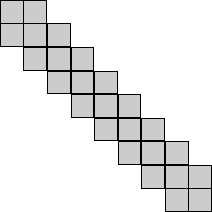
\includegraphics[scale = 1]{figure4_1.pdf} \end{pmatrix} \, \]
    	\caption{An illustration of the sparsity pattern that is present in the smoothing problem.}
	\label{fig:oriEst-sparsity}
\end{figure}

In case the functions $e_i(x_{1:N})$ would be linear, the problem~\eqref{eq:oriEst-generalNLS} would be a \emph{\gls{ls}} problem for which the update~\eqref{eq:oriEst-GNiteration} directly leads to the minimum of the objective function, irrespective of the initial point. In our case where the functions $e_i(x_{1:N})$ are nonlinear due to the nonlinear nature of the orientation, the problem~\eqref{eq:oriEst-generalNLS} is instead a \emph{\gls{nls}} problem. Each iteration in~\eqref{eq:oriEst-GNiteration} can be interpreted as solving a \gls{ls} problem around a linearization point. The linearization point is updated after each iteration, bringing it closer to the minimum of the objective function. Computing an estimate $\hat x_{1:N}$ by iterating~\eqref{eq:oriEst-GNiteration} until convergence, making use of the approximate Hessian from~\eqref{eq:oriEst-approxHessian}, is called \emph{Gauss-Newton optimization}.

Note that since the inertial sensors sample at high sampling rates, the length of the vector $x_{1:N}$ quickly becomes fairly large. For instance, for inertial sensors sampling at $100\hertz$ for $10$ seconds, $N = 1 \thinspace 000$ and the size of the (approximate) Hessian $\mathcal{\hat{H}}(x)$ is $1 \thinspace 000 n_x \times 1 \thinspace 000 n_x$, where $n_x$ is the length of the vector $x_t$. However, as can be seen in~\eqref{eq:oriEst-optNegLogLik}, the components of the objective function only depend on the current and next time steps $x_t$ and $x_{t+1}$. Hence, the structure of the Hessian~\eqref{eq:oriEst-approxHessian} is of the form given in \Figureref{fig:oriEst-sparsity}. There exist efficient algorithms to compute search directions for problems with this sparsity pattern, which can be exploited using sparse matrix packages, see \eg \cite{davis:2006}, or by using tools like dynamic programming and message passing~\citep{bertsekas:1995,golubvL:2013,saad:2003}.

\subsection{Smoothing estimates of the orientation using optimization}
In this section, we will illustrate the use of Gauss-Newton optimization to obtain smoothing estimates of the orientation. As discussed in the previous section, the crucial part is to identify the objective function and its Jacobian. From this, the gradient and approximate Hessian can be computed using~\eqref{eq:oriEst-gradient} and~\eqref{eq:oriEst-approxHessian}, which can be used to iteratively update the estimates using~\eqref{eq:oriEst-GNiteration}. 

Combining the general formulation of the smoothing problem~\eqref{eq:oriEst-optNegLogLik} and using the model for orientation estimation~\eqref{eq:models-ssOri}, the orientation smoothing problem is given by 
\begin{align}
\label{eq:oriEst-oriSmoothing}
\hat{x}_{1:N} = \argmin_{x_{1:N}} &\underbrace{\vphantom{\sum_{t = 2}^N} \| e_{\oriError,\text{i}} \|_{\Sigma_{\oriError,\text{i}}^{-1}}^2}_{\text{Prior}} + \underbrace{\sum_{t = 2}^N \| e_{\omega,t} \|_{\Sigma_\omega^{-1}}^2}_{\text{Dynamics}} + 
\underbrace{\sum_{t = 2}^N \left( \| e_{\text{a},t} \|_{\Sigma_\text{a}^{-1}}^2 + \| e_{\text{m},t} \|_{\Sigma_\text{m}^{-1}}^2\right)}_{\text{Measurement models}},
\end{align}
with
\begin{subequations}
\label{eq:oriEst-smoothingTerms}
\begin{align}
e_{\oriError,\text{i}} &=  2 \logq \left( q_1^\text{nb} \odot \initEst{q}_1^\text{bn} \right), \quad & e_{\oriError,\text{i}} &\sim \mathcal{N}(0,\Sigma_{\oriError,\text{i}}), \\
e_{\omega,t} &= \tfrac{2}{T} \logq \left( q_t^\text{bn} \odot q^\text{nb}_{t+1}\right) - y_{\omega,t}, \quad & e_{\omega,t} &\sim \mathcal{N}(0,\Sigma_\omega),  \\
e_{\text{a},t} &= y_{\text{a},t} + R^\text{bn}_t g^\text{n}, \quad & e_{\text{a},t} &\sim \mathcal{N}(0,\Sigma_\text{a}), \\
e_{\text{m},t} &= y_{\text{m},t} - R^\text{bn}_t m^\text{n}, \quad & e_{\text{m},t} &\sim \mathcal{N}(0,\Sigma_\text{m}). 
\end{align}
\end{subequations}

Convex equality constraints can straightforwardly be incorporated in optimization problems. However, using $N$ equality constraints to preserve the unit norm of the quaternions, severely complicates the optimization problem since these norm constraints are non-convex. Instead, we encode an orientation in terms of a linearization point parametrized as a unit quaternion $\tilde{q}^\text{nb}_t$ and an orientation deviation parametrized as a rotation vector $\oriError_t^\text{n}$ as discussed in \Sectionref{sec:models-linearization}. Hence, we model the orientation as 
\begin{align}
q^\text{nb}_t = \expq \left( \tfrac{\oriError_t^\text{n}}{2} \right) \odot \tilde{q}^\text{nb}_t.
\label{eq:oriEst-linSmoothing}
\end{align}
At each Gauss-Newton iteration~\eqref{eq:oriEst-GNiteration}, we estimate the state vector $\oriError_{1:N}^\text{n}$. Before starting the next iteration, the linearization points $\tilde{q}^\text{nb}_{1:N}$ are updated and the state vector $\oriError_{1:N}^\text{n}$ is reset to zero.

Using the notation introduced in \Sectionref{sec:models-linearization}, the objective function~\eqref{eq:oriEst-oriSmoothing} can be expressed in terms of the orientation deviation $\oriError_t^\text{n}$ by rewriting~\eqref{eq:oriEst-smoothingTerms} as
\begin{subequations}
\label{eq:oriEst-cost}
\begin{align}
e_{\oriError,\text{i}} &=  2 \logq \left( \expq (\tfrac{\eta_{1}^\text{n}}{2}) \odot \tilde{q}_1^\text{nb} \odot \initEst{q}_1^\text{bn} \right), \\
e_{\omega,t} &= \tfrac{2}{T} \logq \left( (\tilde{q}_t^\text{bn} \odot \expq( {\tfrac{\oriError_t^\text{n}}{2}}) )^\conj \odot \expq ({\tfrac{\oriError_{t+1}^\text{n}}{2}}) \odot \tilde{q}^\text{nb}_{t+1} \right) - y_{\omega,t}, \\
e_{\text{a},t} &= y_{\text{a},t} + \tilde{R}^\text{bn}_t \left( \expR( \oriError_t^\text{n} ) \right)^\Transp g^\text{n}, \label{eq:oriEst-costAcc} \\
e_{\text{m},t} &= y_{\text{m},t} - \tilde{R}^\text{bn}_t \left( \expR( \oriError_t^\text{n} ) \right)^\Transp m^\text{n}. \label{eq:oriEst-costMag}
\end{align}
\end{subequations}
Here, $\tilde{R}^\text{bn}_t$ is the rotation matrix representation of the linearization point $\tilde{q}^\text{bn}_t$. This leads to the following derivatives
\begin{subequations}
\label{eq:oriEst-der}
\begin{align}
\tfrac{\diff e_{\oriError,\text{i}} }{\diff \oriError_{1}^\text{n}}  &=  \tfrac{\diff \logq (q)}{\diff q} \left( \tilde{q}^\text{nb}_{1} \odot \initEst{q}_1^\text{bn}\right)^\rightMult \tfrac{\diff \expq (\oriError_{1}^\text{n})}{\diff \oriError_{1}^\text{n}}, \label{eq:oriEst-derInit} \\
\tfrac{\diff e_{\omega,t} }{\diff \oriError_{t+1}^\text{n}} &= \tfrac{1}{T} \tfrac{\diff \logq (q)}{\diff q} \left( \tilde{q}_t^\text{bn} \right)^\leftMult \left( \tilde{q}^\text{nb}_{t+1}\right)^\rightMult \tfrac{\diff \expq (\oriError_{t+1}^\text{n})}{\diff \oriError_{t+1}^\text{n}}, \label{eq:oriEst-derDynModelNow} \\
\tfrac{\diff e_{\omega,t} }{\diff \oriError_t^\text{n}} &= \tfrac{1}{T} \tfrac{\diff \logq (q)}{\diff q} \left( \tilde{q}_t^\text{bn} \right)^\leftMult \left( \tilde{q}^\text{nb}_{t+1} \right)^\rightMult \tfrac{\diff \left( \expq  (\oriError_{t}^\text{n}) \right)^\conj}{\diff \expq (\oriError_{t}^\text{n})} \tfrac{\diff \expq (\oriError_{t}^\text{n})}{\diff \oriError_{t}^\text{n}}, \label{eq:oriEst-derDynModelPrev} \\
\tfrac{\diff e_{\text{a},t} }{\diff \oriError_t^\text{n}}&\approx \tilde{R}^\text{bn}_t [g^\text{n} \times], \label{eq:oriEst-derAcc} \\
\tfrac{\diff e_{\text{m},t} }{\diff \oriError_t^\text{n}} &\approx - \tilde{R}^\text{bn}_t [m^\text{n} \times], \label{eq:oriEst-derMag}
\end{align}
\end{subequations}
where, using~\eqref{eq:models-logexpq-approx} and the definition of the quaternion conjugate~\eqref{eq:models-quatConj}, 
\begin{align}
\tfrac{\diff \logq (q)}{\diff q} &\approx \begin{pmatrix} 0_{1 \times 3} \\ \mathcal{I}_3 \end{pmatrix}^\Transp, \qquad
\tfrac{\diff \left( \expq (\oriError) \right)^\conj}{\diff \exp \oriError} = \begin{pmatrix} 1 & 0_{1 \times 3} \\ 0_{3 \times 1} & - \mathcal{I}_3 \end{pmatrix}, \nonumber \\
\tfrac{\diff \expq \oriError}{\diff \oriError} &\approx \begin{pmatrix} 0_{1 \times 3} \\ \mathcal{I}_3 \end{pmatrix}.
\end{align}
Using the approximate derivatives~\eqref{eq:oriEst-der}, the gradient and approximate Hessian can be computed for the Gauss-Newton iterations. The resulting solution is summarized in \Algorithmref{alg:oriEst-smoothingOpt}. One of the inputs to the algorithm is an initial estimate of the orientation $\tilde{q}^{\text{nb},(0)}_{1:N}$, which will aid the convergence to the desired minimum. There are (at least) two ways to obtain good initial estimates $\tilde{q}^{\text{nb},(0)}_{1:N}$. First, they can be obtained by direct integration of the gyroscope measurements. As discussed in \Sectionref{sec:intro-imusForPose}, these estimates will suffer from integration drift. However, they still form a good initial estimate for the optimization problem. Second, one of the other, computationally cheaper estimation algorithms that will be discussed in the remainder of this section can be used to obtain initial estimates of the orientation.

\begin{algorithm}[htp]
\caption{\textsf{Smoothing estimates of the orientation using optimization}}
\label{alg:oriEst-smoothingOpt}
\small
\textsc{Inputs:} An initial estimate of the orientation $\tilde{q}^{\text{nb},(0)}_{1:N}$, inertial data $\left\{ y_{\text{a},t}, y_{\omega,t} \right\}_{t=1}^N$, magnetometer data $\left\{ y_{\text{m},t}\right\}_{t=1}^N$ and covariance matrices $\Sigma_\omega$, $\Sigma_\text{a}$ and $\Sigma_\text{m}$. \\
\textsc{Outputs:} An estimate of the orientation $\hat{q}^\text{nb}_{1:N}$ and optionally its covariance $\cov (\hat{\oriError}^\text{n}_{1:N})$.
\algrule[.4pt]
\begin{enumerate}
\item Set $\hat \oriError_t^{\text{n},(0)} = 0_{3 \times 1}$ for $t = 1, \hdots, N$, set $k = 0$ and compute $\initEst{q}_1^\text{nb}$ and $\Sigma_{\oriError,\text{i}}$ as described in \Sectionref{sec:models-prior}.
\item \textbf{while} \textit{termination condition is not satisfied} \textbf{do}
\begin{enumerate}
\item Compute the gradient~\eqref{eq:oriEst-gradient} and the approximate Hessian~\eqref{eq:oriEst-approxHessian} of the orientation smoothing problem~\eqref{eq:oriEst-oriSmoothing} using the expressions for the different parts of the cost function and their Jacobians~\eqref{eq:oriEst-cost} and~\eqref{eq:oriEst-der}.
\item Apply the update~\eqref{eq:oriEst-GNiteration} to obtain $\hat \oriError_{1:N}^{\text{n},(k+1)}$.
\item Update the linearization point as
\begin{align}
\tilde q^{\text{nb},(k+1)}_t = \expq \left( \tfrac{\hat{\oriError}_t^{\text{n},(k+1)}}{2} \right) \odot \tilde{q}^{\text{nb},(k)}_t,
\label{eq:oriEst-relinSmoothing}
\end{align}
and set $\hat \oriError_t^{\text{n},(k+1)} = 0_{3 \times 1}$ for $t = 1, \hdots, N$.
\item Set $k = k+1$.
\end{enumerate}
\item[] \textbf{end while}
\item Set $\hat{q}^\text{nb}_{1:N} = \tilde{q}^{\text{nb},(k)}_{1:N}$.
\item Optionally compute
\begin{align}
\cov (\hat{\oriError}^\text{n}_{1:N}) = \left( \mathcal{J}^\Transp(\hat{\oriError}^\text{n}_{1:N}) \mathcal{J} (\hat{\oriError}^\text{n}_{1:N}) \right)^{-1}.
\end{align}
\end{enumerate}
\normalsize
\end{algorithm}

\subsection{Computing the uncertainty}
\label{sec:oriEst-smoothingUncertainty}
As discussed in \Sectionref{sec:models-probModeling}, we are not only interested in obtaining point estimates of the position and orientation, but also in estimating their uncertainty. In our case of Gaussian noise, this is characterized by the covariance. As shown in \eg \cite{ljung:1999,verhaegenV:2007}, if our position and orientation estimation problems would be \gls{ls} problems, the covariance of the estimates would be given by the inverse of the Hessian of the objective function~\eqref{eq:oriEst-hessian}. Instead, we solve an \gls{nls} problem, for which a number of \gls{ls} problems are solved around linearization points closer and closer to the minimum of the objective function. Hence, when the algorithm has converged, the problem can locally well be described by the quadratic approximation around its resulting linearization point. We can therefore approximate the covariance of our estimates as
\begin{align}
\cov{ (\hat{x}_{1:N}) } = \left( \mathcal{J}^\Transp(\hat{x}_{1:N}) \mathcal{J}(\hat{x}_{1:N}) \right)^{-1}.
\end{align}
An intuition behind this expression is that the accuracy of the estimates is related to the sensitivity of the objective function with respect to the states. The covariance of the estimate will play a crucial role in the filtering approaches discussed in \Sectionref{sec:oriEst-filteringOpt} and~\Sectionref{sec:oriEst-ekf}.

The matrix $\mathcal{J}^\Transp(\hat{x}_{1:N}) \mathcal{J}(\hat{x}_{1:N})$ quickly becomes fairly large due to the high sampling rates of the inertial sensors. Hence, computing its inverse can be computationally costly. We are, however, typically only interested in a subset of the inverse. For instance, we are often only interested in diagonal or block diagonal elements representing $\cov (x_t)$. It is therefore not necessary to explicitly form the complete inverse, which makes the computation tractable also for larger problem sizes.

\section{Filtering estimation in an optimization framework}
\label{sec:oriEst-filteringOpt}
One of the benefits of using a smoothing formulation is that all measurements $y_{1:N}$ are used to get the best estimates of the states $x_{1:N}$. However, both the computational cost and the memory requirements grow with the length of the data set. Furthermore, it is a post-processing solution in which we have to wait until all data is available. Alternatively, the filtering problem can be formulated as 
\begin{align}
\label{eq:oriEst-filtOpt}
\hat{x}_{t+1} &= \argmin_{x_{t+1}} - \log p(x_{t+1} \mid y_{1:t+1}) \nonumber \\
&= \argmin_{x_{t+1}} - \log p(y_{t+1} \mid x_{t+1}) - \log p(x_{t+1} \mid y_{1:t}).
\end{align}
Note that without loss of generality, we have shifted our time indices as compared to the notation in \Sectionref{sec:models-probModeling}. The probability distribution $p(x_{t+1} \mid y_{1:t})$ can now be seen as a \emph{prior} and can be obtained by marginalizing out the previous state $x_{t}$ as
\begin{align}
\label{eq:oriEst-filteringOptMargDistr}
p(x_{t+1}  \mid y_{1:t}) &= \int p(x_{t+1} , x_{t} \mid y_{1:t} ) \dint x_{t} \nonumber \\
&= \int p(x_{t+1} \mid x_{t}) p(x_{t} \mid y_{1:t}) \dint x_{t}.
\end{align}
Assuming that
\begin{subequations}
\begin{align}
p(x_{t+1} \mid x_{t}) &\sim \mathcal{N}( x_{t+1} \, ; \, f(x_{t}), Q),  \\
p(x_{t} \mid y_{1:t}) &\sim \mathcal{N}( x_{t} \, ; \, \hat{x}_{t}, P_{t \mid t}),
\end{align}
\end{subequations}
the integral in~\eqref{eq:oriEst-filteringOptMargDistr} can be approximated as
\begin{align}
\label{eq:oriEst-filteringOptMargDistr-approx}
p(x_{t+1} \mid y_{1:t}) &\approx \mathcal{N}\left( x_{t+1} \, ; \,  f(\hat{x}_{t}), F_{t} P_{t \mid t} F_{t}^\Transp + G_{t} Q G_{t}^\Transp \right).
\end{align}
Here, $F_{t} = \givenThat{\tfrac{\partial f(x_{t})}{\partial x_{t}}}{x_t = \hat{x}_t}{w_t = 0}$, $\givenThat{G_{t} = \tfrac{\partial f(x_{t})}{\partial w_{t}}}{x_t = \hat{x}_t}{w_t = 0}$ and $w_t$ is the process noise defined in~\eqref{eq:models-dynamics}. Using~\eqref{eq:oriEst-filteringOptMargDistr-approx}, the filtering problem~\eqref{eq:oriEst-filtOpt} can again be written as a nonlinear least squares problem and can be solved using Gauss-Newton optimization as described in \Sectionref{sec:oriEst-GNopt}. Instead of optimizing over the whole data set at once as in \Sectionref{sec:oriEst-smoothingOpt}, we solve a small optimization problem at each time instance $t$. This is closely related to what is often called an iterated extended Kalman filter~\cite{jazwinski:1970,skoglundHA:2015}.

\subsection{Filtering estimates of the orientation using optimization}
\label{sec:oriEst-filteringOpt-ori}
In this section, we will derive an algorithm to obtain filtering estimates of the orientation using Gauss-Newton optimization. The resulting algorithm is closely related to the iterated multiplicative extended Kalman filter presented in \cite{skoglundSK:2017}.

To derive the approximation~\eqref{eq:oriEst-filteringOptMargDistr-approx} for the orientation estimation problem, we first derive an expression for the function $f$ that expresses $\oriError_{t+1}^\text{n}$ in terms of $\oriError^\text{n}_{t}$. Using~\eqref{eq:oriEst-linSmoothing} in combination with~\eqref{eq:models-ssOri-dyn}, 
\begin{align}
\oriError^\text{n}_{t+1} &= f(\oriError^\text{n}_{t}, y_{\omega,t}, e_{\omega,t}) \\ 
&= 2 \logq \left( \expq(\tfrac{\oriError^\text{n}_{t}}{2}) \odot \tilde{q}_{t}^\text{nb} \odot \expq \left(\tfrac{T}{2} (y_{\omega,t} + e_{\omega,t} ) \right) \odot \tilde{q}_{t+1}^\text{bn} \right). \nonumber
\label{eq:oriEst-filtOptCost}
\end{align}
Here, $\oriError^\text{n}_{t}$ and $\tilde{q}_{t}^\text{nb}$ provide information about the previous time step. We denote the orientation estimate from the previous time step as $\hat{q}_{t}^\text{nb}$ and assume that $\hat{\oriError}_t^\text{n}$ is zero since the linearization point is updated after each iteration of the optimization algorithm. To start with a fairly good linearization point, we choose $\tilde{q}_{t+1}^{\text{nb},(0)}$ at iteration $k = 0$ as
\begin{align}
\tilde{q}_{t+1}^{\text{nb},(0)} = \hat{q}_{t}^\text{nb} \odot \expq \left( \tfrac{T}{2} y_{\omega,t} \right).
\end{align}
Following~\eqref{eq:oriEst-filteringOptMargDistr-approx}, the distribution $p(\oriError^\text{n}_{t+1} \mid y_{1:t})$ around this linearization point can now be written as
\begin{align}
\label{eq:oriEst-filtOptDist}
p(\oriError^\text{n}_{t+1} \mid y_{1:t}) &\approx \mathcal{N}\left( \oriError^\text{n}_{t+1} \, ; \, 0, F_{t} P_{t \mid t} F_{t}^\Transp + G_{t} \Sigma_\omega G_{t}^\Transp \right),
\end{align}
with 
\begin{subequations}
\label{eq:oriEst-filtOptFG}
\begin{align}
F_{t} &= \givenThat{\tfrac{\partial f(\oriError^\text{n}_{t},y_{\omega,t},e_{\omega,t})}{\partial \oriError^\text{n}_{t}}}{\oriError^\text{n}_{t} = 0, \tilde{q}_{t}^\text{nb} = \hat{q}_{t}^\text{nb}}{e_{\omega,t} = 0} \nonumber \\
&= 2 \left. \tfrac{\partial}{\partial \oriError^\text{n}_{t}}  \logq \left( \expq(\tfrac{\oriError^\text{n}_{t}}{2}) \right) \right|_{\oriError^\text{n}_{t} = 0} \nonumber \\
&= \mathcal{I}_3, \label{eq:oriEst-filtOptDynF} \\
G_{t} &= \givenThat{\tfrac{\partial f(\oriError^\text{n}_{t},y_{\omega,t},e_{\omega,t})}{\partial e_{\omega,t}}}{\oriError^\text{n}_{t} = 0, \tilde{q}_{t}^\text{nb} = \hat{q}_{t}^\text{nb}}{e_{\omega,t} = 0} \nonumber \\
&= 2 \left. \tfrac{\partial}{\partial e_{\omega,t}}   \logq \left( \hat{q}_{t}^\text{nb} \odot \expq \left(\tfrac{T}{2} (y_{\omega,t} + e_{\omega,t} ) \right) \right. \right. \nonumber \\
& \qquad \qquad \left. \left. \odot \expq \left(-\tfrac{T}{2} y_{\omega,t} \right) \odot \hat{q}_{t}^\text{bn} \right) \right|_{e_{\omega,t} = 0} \nonumber \\
&\approx T \tilde{R}_{t+1}^{\text{nb},(0)}.
\end{align}
\end{subequations}

The covariance $P_{t \mid t}$ in~\eqref{eq:oriEst-filtOptDist} can be approximated as the inverse of the Hessian of the objective function from the previous time step, see also \Sectionref{sec:oriEst-smoothingUncertainty}. We make use of the shorthand notation $P_{t+1 \mid t} = F_{t} P_{t \mid t} F_{t}^\Transp + G_{t} Q G_{t}^\Transp$ and define
\begin{align}
\label{eq:oriEst-costDerFiltMarg}
e_{\text{f},t} = \oriError^\text{n}_{t}- 2 \logq \left(\hat{q}_{t-1}^\text{nb} \odot \expq (\tfrac{T}{2} y_{\omega,t-1} ) \odot  \tilde{q}_{t}^\text{bn} \right), 
\qquad \tfrac{\diff e_{\text{f},t}}{\diff \oriError^\text{n}_{t}} &= \mathcal{I}_3.
\end{align}
Note that $e_{\text{f},t}$ is equal to zero for iteration $k = 0$ but can be non-zero for subsequent iterations. Using this notation, the filtering problem~\eqref{eq:oriEst-filtOpt} results in the following optimization problem
\begin{align}
\label{eq:oriEst-filtOptNLS}
\hat{x}_t &= \argmin_{x_{t}} - \log p(x_{t} \mid y_{1:t}) \nonumber \\
&= \argmin_{x_{t}} \underbrace{\| e_{\text{f},t} \|_{P_{t \mid t-1}^{-1}}}_{\begin{subarray}{c}\text{Dynamics and}\\
    \text{knowledge about $x_{t-1}$}\end{subarray}} + \underbrace{\vphantom{\| e_{\text{f},t} \|_{P_{t \mid t-1}^{-1}}} \| e_{\text{a},t} \|_{\Sigma_\text{a}^{-1}} + \| e_{\text{m},t} \|_{\Sigma_\text{m}^{-1}}}_{\text{Measurement models}}.
\end{align}
Note the similarity of this optimization problem to the smoothing formulation in~\eqref{eq:oriEst-oriSmoothing}. The term $\| e_{\text{f},t} \|_{P_{t \mid t-1}^{-1}}$ takes into account both the knowledge about the previous state $x_t$ and the dynamics. Furthermore, due to the fact that $P_{t \mid t-1}^{-1}$ is time-varying, the uncertainty and cross-correlation of the states at the previous time instance is taken into consideration. Including this term is similar to the inclusion of an arrival cost in moving horizon estimation approaches~\citep{raoRM:2003}.

After each Gauss-Newton iteration, we need to recompute the linearization point as
\begin{align}
\label{eq:oriEst-filtOptRelinCov}
\tilde{q}_{t}^{\text{nb},(k+1)} &= \expq \left( \tfrac{\hat{\oriError}_t^{\text{n},(k+1)}}{2} \right) \odot \tilde{q}_{t}^{\text{nb},(k)}.
\end{align}
We also need to compute the covariance around this updated linearization point as
\begin{align}
P_{t \mid t-1}^{(k+1)} &= J_{t}^{(k)} P_{t \mid t-1}^{(k)} \left( J_{t}^{(k)} \right)^\Transp,
\end{align}
where $J_t^{(k)}$ can be derived similarly to the derivation of~$F_t$ in~\eqref{eq:oriEst-filtOptDynF}. Since $J_t^{(k)} = \mathcal{I}_3$, in practice the relinearization of the covariance can be omitted. The process of estimating orientation using filtering is summarized in \Algorithmref{alg:oriEst-filteringOpt}.

\begin{algorithm}[ht]
\caption{\textsf{Filtering estimates of the orientation using optimization}}
\label{alg:oriEst-filteringOpt}
\small
\textsc{Inputs:} Inertial data $\left\{ y_{\text{a},t}, y_{\omega,t} \right\}_{t=1}^N$, magnetometer data $\left\{ y_{\text{m},t}\right\}_{t=1}^N$ and covariance matrices $\Sigma_\omega$, $\Sigma_\text{a}$ and $\Sigma_\text{m}$. \\
\textsc{Outputs:} An estimate of the orientation $\hat{q}^\text{nb}_{t}$ and its covariance $P_{t \mid t}$ for $t = 1, \hdots N$.
\algrule[.4pt]
\begin{enumerate}
\item Compute $\initEst{q}_1^\text{nb}$ and $\Sigma_\text{i}$ as described in \Sectionref{sec:models-prior} and set $\hat{q}_{1}^\text{nb} = \initEst{q}_{1}^\text{nb}$ and $P_{1 \mid 1} = \Sigma_{\oriError,\text{i}}$.
\item \textbf{for} $t = 2, \hdots N$ \textbf{do}
\begin{enumerate}
\item Set $\hat \oriError_t^{\text{n},(0)} = 0_{3 \times 1}$, set $k = 0$, choose the linearization point $\tilde q^{\text{nb},(0)}_t$ as
\begin{subequations}
\begin{align}
\label{eq:oriEst-filteringOpt-updateLinPointIt0}
\tilde q^{\text{nb},(0)}_t &= \hat{q}^{\text{nb}}_{t-1} \odot \expq \left( \tfrac{T}{2} y_{\omega,t-1} \right), \\
\intertext{and compute $P_{t \mid t-1}$ as}
P_{t \mid t-1} &= P_{t-1 \mid t-1} + G_{t-1} \Sigma_\omega G_{t-1}^\Transp,
\label{eq:oriEst-timeUpdateFiltOpt}
\end{align}
\end{subequations}
with $G_{t-1} = T \tilde{R}^{\text{nb},(0)}_{t}$.
\item \textbf{while} \textit{termination condition is not satisfied} \textbf{do}
\begin{enumerate}
\item Compute the gradient~\eqref{eq:oriEst-gradient} and the approximate Hessian~\eqref{eq:oriEst-approxHessian} of the filtering problem~\eqref{eq:oriEst-filtOptNLS} using the expressions for the different parts of the cost function and their Jacobians~\eqref{eq:oriEst-costDerFiltMarg},~\eqref{eq:oriEst-costAcc},~\eqref{eq:oriEst-costMag},~\eqref{eq:oriEst-derAcc} and~\eqref{eq:oriEst-derMag}.
\item Apply the update~\eqref{eq:oriEst-GNiteration} to obtain $\hat \oriError_{t}^{\text{n},(k+1)}$.
\item Update the linearization point as 
\begin{align}
\tilde q^{\text{nb},(k+1)}_t &= \expq \left( \tfrac{\hat{\oriError}_t^{\text{n},(k+1)}}{2} \right) \odot \tilde{q}^{\text{nb},(k)}_t, 
\label{eq:oriEst-relinFiltering}
\end{align}
$\hat \oriError_t^{\text{n},(k+1)} = 0_{3 \times 1}$.
\item Set $k = k+1$.
\end{enumerate}
\item[] \textbf{end while}
\item Set $\hat{q}^\text{nb}_{t} = \tilde{q}^{\text{nb},(k)}_{t}$, $\hat{\oriError}^\text{n}_{t} = \hat{\oriError}^{\text{n},(k)}_{t}$ and compute $P_{t \mid t}$ as
\begin{align}
P_{t \mid t} = \left( \mathcal{J}^\Transp(\hat{\oriError}^\text{n}_{t}) \mathcal{J}(\hat{\oriError}^\text{n}_{t}) \right)^{-1}.
\end{align}
\end{enumerate}
\end{enumerate}
\normalsize
\end{algorithm}

\section{Extended Kalman filtering}
\label{sec:oriEst-ekf}
Instead of using optimization for position and orientation estimation, it is also possible to use extended Kalman filtering. \Glspl{ekf} compute filtering estimates in terms of the conditional probability distribution~\eqref{eq:models-filtering}. Hence, the approach is similar to the one discussed in \Sectionref{sec:oriEst-filteringOpt}. In fact, extended Kalman filtering can be interpreted as Gauss-Newton optimization of the filtering problem using only one iteration~\eqref{eq:oriEst-GNiteration} with a step length of one, see \eg \cite{skoglundHA:2015}. In this section we first introduce how an \gls{ekf} can be used to compute state estimates in a general nonlinear state space model. Subsequently, we illustrate the use of \glspl{ekf} for position and orientation estimation by focusing on the orientation estimation problem. Two different implementations will be discussed. First, we introduce an \gls{ekf} implementation that uses unit quaternions as states. Subsequently, we discuss an \gls{ekf} which parametrizes the orientation in terms of an orientation deviation from a linearization point, similar to the approach used in \Sectionref{sec:oriEst-smoothingOpt} and~\Sectionref{sec:oriEst-filteringOpt}. 

An \gls{ekf} makes use of a nonlinear state space model. Assuming that the measurement noise is additive and that both the process and the measurement noise are zero-mean Gaussian with constant covariance, the state space model is given by
\begin{subequations}
\begin{align}
x_{t+1} &= f_t(x_t,u_t,w_t), \label{eq:oriEst-generalSSmodel-dyn} \\
y_t &= h_t(x_t) + e_t, \label{eq:oriEst-generalSSmodel-meas}
\end{align}
\label{eq:oriEst-generalSSmodel}%
\end{subequations}%
with $w_t \sim \mathcal{N}(0,Q)$ and $e_t \sim \mathcal{N}(0,R)$.

The state is estimated recursively by performing a \emph{time update} and a \emph{measurement update}. The time update uses the model~\eqref{eq:oriEst-generalSSmodel-dyn} to ``predict'' the state to the next time step according to 
\begin{subequations}
\begin{align}
\hat{x}_{t+1 \mid t} &= f_t(\hat{x}_{t \mid t},u_t), \label{eq:ekfTxupdate} \\
P_{t+1 \mid t} &= F_t P_{t \mid t} F_t^\Transp + G_t Q G_t^\Transp, \label{eq:ekfTPupdate}
\end{align}
\label{eq:oriEst-ekfTimeUpdate}%
\end{subequations}%
with 
\begin{align}
F_t = \givenThat{\tfrac{\partial f_t(x_t,u_t,w_t)}{\partial x_t}}{x_t=\hat{x}_{t \mid t}}{w_t=0}, \qquad G_t = \givenThat{\tfrac{\partial f_t(x_t,u_t,w_t)}{\partial v_t}}{x_t=\hat{x}_{t \mid t}}{w_t=0}.
\label{eq:oriEst-defFG}
\end{align}
Here, the matrix $P$ denotes the state covariance. The double subscripts on $\hat{x}_{t+1 \mid t}$ and $P_{t+1 \mid t}$ denote the state estimate and the state covariance at time $t+1$ given measurements up to time $t$. Similarly, $\hat{x}_{t \mid t}$ and $P_{t \mid t}$ denote the state estimate and the state covariance at time $t$ given measurements up to time $t$. 

The measurement update makes use of the measurement model \eqref{eq:oriEst-generalSSmodel-meas} in combination with the measurements $y_t$ to update the ``predicted'' state estimate as 
\begin{subequations}
\begin{align}
\hat{x}_{t \mid t} &= \hat{x}_{t \mid t-1} + K_t \varepsilon_t, \label{eq:ekfMxupdate} \\
P_{t \mid t} &= P_{t \mid t-1} - K_t S_t K_t^\Transp, \label{eq:ekfMPupdate}
\end{align}
\label{eq:oriEst-ekfMeasUpdate}%
\end{subequations}%
with
\begin{align}
\label{eq:oriEst-defEpsKS}
\varepsilon_t \triangleq y_t - \hat{y}_{t \mid t-1}, \, \, \, \, S_t \triangleq H_t P_{t \mid t-1} H_t^\Transp + R, \, \, \, \, K_t \triangleq P_{t \mid t-1} H_t^\Transp S_t^{-1},
\end{align}
and
\begin{align}
\label{eq:oriEst-defYhatH}
\hat{y}_{t \mid t-1} = h(\hat{x}_{t \mid t-1}), \qquad H_t = \left. \tfrac{\partial h_t(x_t)}{\partial x_t} \right|_{x_t=\hat{x}_{t \mid t-1}}.
\end{align}
Note that in~\eqref{eq:oriEst-ekfMeasUpdate} we have shifted our notation one time step compared to the notation in~\eqref{eq:oriEst-ekfTimeUpdate} to avoid cluttering the notation. The \gls{ekf} iteratively performs a time update and a measurement update to estimate the state and its covariance.

\subsection{Estimating orientation using quaternions as states}
\label{sec:oriEst-quat-ekf}
In this section, we will illustrate the use of an \gls{ekf} to compute filtering estimates of the orientation. As discussed in the previous section, the crucial part is to compute the matrices $F_t$, $G_t$ and $H_t$ to perform the \gls{ekf} time and measurement updates. Using the state space model~\eqref{eq:models-ssOri} and using unit quaternions as states in the \gls{ekf}, the dynamic model is given by 
\begin{align}
q^\text{nb}_{t+1} &= f_t(q^\text{nb}_t,y_{\omega,t},e_{\omega,t}) = q^\text{nb}_t \odot \expq \left(\tfrac{T}{2} ( y_{\omega,t} - e_{\omega,t} ) \right) \nonumber \\
&= \left( \expq \left(\tfrac{T}{2} ( y_{\omega,t} - e_{\omega,t} ) \right) \right)^\rightMult q^{\text{nb}}_t \nonumber \\
&= \left( q^\text{nb}_t \right)^\leftMult \expq \left(\tfrac{T}{2} ( y_{\omega,t} - e_{\omega,t} ) \right).
\label{eq:oriEst-quatEKF-dyn}
\end{align}
The following derivatives of the dynamic model~\eqref{eq:oriEst-quatEKF-dyn} can be obtained
\begin{subequations}
\begin{align}
F_t &= \givenThat{\tfrac{\partial f_t(q^\text{nb}_t,y_{\omega,t},e_{\omega,t})}{\partial q^\text{nb}_t}}{q^\text{nb}_{t}=\hat{q}^\text{nb}_{t \mid t}}{e_{\omega,t}=0} = \left( \expq (\tfrac{T}{2} y_{\omega,t} ) \right)^\rightMult, \\
G_t &= \givenThat{\tfrac{\partial f_t(q^\text{nb}_t,y_{\omega,t},e_{\omega,t})}{\partial e_{\omega,t}}}{q^\text{nb}_{t}=\hat{q}^\text{nb}_{t \mid t}}{e_{\omega,t}=0} \nonumber \\
&= \givenThat{\tfrac{\partial}{\partial e_{\omega,t}} \left( q^{\text{nb}}_t \right)^\leftMult \expq ( \tfrac{T}{2} ( y_{\omega,t} - e_{\omega,t} )) }{q^\text{nb}_{t}=\hat{q}^\text{nb}_{t \mid t}}{e_{\omega,t}=0} \nonumber \\
&= -\tfrac{T}{2} \left( \hat{q}^{\text{nb}}_{t \mid t} \right)^\leftMult \tfrac{\diff \expq (e_{\omega,t})}{\diff e_{\omega,t}}.
\end{align}
\end{subequations}

In the measurement update of the \gls{ekf}, the state is updated using the accelerometer and magnetometer measurements. Using the measurement models
\begin{align}
y_{\text{a},t} = - R^\text{bn}_t g^\text{n} + e_{\text{a},t}, \qquad y_{\text{m},t} = R^\text{bn}_t m^\text{n} + e_{\text{m},t},
\end{align}
the matrix $H_t$ in~\eqref{eq:oriEst-defYhatH} is given by
\begin{align}
H_t &= \left. \tfrac{\partial}{\partial q^\text{nb}_t} \begin{pmatrix} R^\text{bn}_t g^\text{n} \\ R^\text{bn}_t m^\text{n} \end{pmatrix} \right|_{q^\text{nb}_t=\hat{q}^\text{nb}_{t \mid t-1}} 
= \begin{pmatrix} - \left. \tfrac{\partial R^\text{bn}_{t \mid t-1}}{\partial q^\text{nb}_{t \mid t-1}} \right|_{q^\text{nb}_{t \mid t-1}=\hat{q}^\text{nb}_{t \mid t-1}} g^\text{n} \\ \left. \tfrac{\partial R^\text{bn}_{t \mid t-1}}{\partial q^\text{nb}_{t \mid t-1}} \right|_{q^\text{nb}_{t \mid t-1}=\hat{q}^\text{nb}_{t \mid t-1}} m^\text{n} \end{pmatrix}.
\end{align}
The derivative $\tfrac{\partial R^\text{bn}_{t \mid t-1}}{\partial q^\text{nb}_{t \mid t-1}}$ can be computed from the definition of the relation between and the rotation matrix and the quaternion representation given in~\eqref{eq:app-defRq}.

Note that the quaternion obtained from the measurement update \eqref{eq:oriEst-ekfMeasUpdate} is no longer normalized. We denote this unnormalized quaternion and its covariance by $\tilde{q}_{t \mid t}^\text{nb}$ and $\tilde{P}_{t \mid t}$, respectively. The $\tilde{\cdot}$ instead of the $\hat{\cdot}$ is meant to explicitly indicate that the quaternion still needs to be updated. This is done by an additional renormalization step as compared to a standard \gls{ekf} implementation. A possible interpretation of the renormalization is as an additional measurement update without measurement noise. Hence, we adjust both the quaternion and its covariance as
\begin{subequations}
\label{eq:oriEst-ekfQuatRenorm}
\begin{align}
\hat{q}_{t \mid t}^\text{nb} &= \tfrac{\tilde{q}^\text{nb}_{t \mid t}}{\| \tilde{q}^\text{nb}_{t \mid t}\|_2},  \qquad
P_{t \mid t} = J_t \tilde{P}_{t \mid t} J_t^\Transp, 
\intertext{with}
J_t &= \tfrac{1}{\| \tilde{q}^\text{nb}_{t \mid t} \|_2^3} \tilde{q}^\text{nb}_{t \mid t} \left( \tilde{q}^\text{nb}_{t \mid t} \right)^\Transp.
\end{align}
\end{subequations}
Here, $q^\Transp$ is the standard vector transpose. The resulting \gls{ekf} is summarized in \Algorithmref{alg:oriEst-ekfQuat}. 

\begin{algorithm}[ht]
\caption{\textsf{Orientation estimation using an EKF with quaternion states}}
\label{alg:oriEst-ekfQuat}
\small
\textsc{Inputs:} Inertial data $\left\{ y_{\text{a},t}, y_{\omega,t} \right\}_{t=1}^N$, magnetometer data $\left\{ y_{\text{m},t}\right\}_{t=1}^N$ and covariance matrices $\Sigma_\omega$, $\Sigma_\text{a}$ and $\Sigma_\text{m}$. \\
\textsc{Outputs:} An estimate of the orientation $\hat{q}^\text{nb}_{t \mid t}$ and its covariance $P_{t \mid t}$ for $t = 1, \hdots N$.
\algrule[.4pt]
\begin{enumerate}
\item Compute $\initEst{q}^\text{nb}_{1}$ and $\Sigma_\text{i}$ as described in \Sectionref{sec:models-prior} and set $\hat{q}_{1 \mid 1}^\text{nb} = \initEst{q}_{1}^\text{nb}$ and $P_{1 \mid 1} = \Sigma_\text{q,i}$.
\item \textbf{For} $t = 2, \hdots, N$ \textbf{do}
\begin{enumerate}
\item Time update
\begin{subequations}
\begin{align}
\hat{q}^\text{nb}_{t \mid t-1} &= \hat{q}^\text{nb}_{t-1 \mid t-1} \odot \expq \left( \tfrac{T}{2} y_{\omega,t-1} \right), \\
P_{t \mid t-1} &= F_{t-1} P_{t-1 \mid t-1} F_{t-1}^\Transp + G_{t-1} Q G_{t-1}^\Transp, \label{eq:quatEKF_TPupdate} %
\end{align}%
\label{eq:ori_qEkf_timeUpdate}%
\end{subequations}%
with $Q = \Sigma_\omega$ and 
\begin{align*}
F_{t-1} = \left( \expq (\tfrac{T}{2} y_{\omega,t-1}) \right)^\rightMult, \, G_{t-1} = -\tfrac{T}{2} \left( \hat{q}^{\text{nb}}_{t-1 \mid t-1} \right)^\leftMult \tfrac{\diff \expq (e_{\omega,t-1})}{\diff e_{\omega,t-1}}.
\end{align*}
\item Measurement update
\begin{subequations}
\begin{align}
\tilde{q}^\text{nb}_{t \mid t} &= \hat{q}^\text{nb}_{t \mid t-1} + K_t \varepsilon_t,  \\
\tilde{P}_{t \mid t} &= P_{t \mid t-1} - K_t S_t K_t^\Transp, 
\end{align}
\label{eq:ori_qEkf_measUpdate}
\end{subequations}%
with $\varepsilon_t$, $K_t$ and $S_t$ defined in~\eqref{eq:oriEst-defEpsKS} and
\begin{align*}
y_t &= \begin{pmatrix} y_{\text{a},t} \\ y_{\text{m},t} \end{pmatrix}, & 
\hat{y}_{t \mid t-1} &= \begin{pmatrix} -\hat{R}^\text{bn}_{t \mid t-1} g^\text{n} \\ \hat{R}^\text{bn}_{t \mid t-1} m^\text{n} \end{pmatrix}, \\
H_t &= \begin{pmatrix} - \left. \tfrac{\partial R^\text{bn}_{t \mid t-1}}{\partial q^\text{nb}_{t \mid t-1}} \right|_{q^\text{nb}_{t \mid t-1}=\hat{q}^\text{nb}_{t \mid t-1}} g^\text{n} \\ \left. \tfrac{\partial R^\text{bn}_{t \mid t-1}}{\partial q^\text{nb}_{t \mid t-1}} \right|_{q^\text{nb}_{t \mid t-1}=\hat{q}^\text{nb}_{t \mid t-1}} m^\text{n} \end{pmatrix}, & 
R &= \begin{pmatrix} \Sigma_\text{a} & 0 \\ 0 & \Sigma_\text{m} \end{pmatrix}.
\end{align*}
\item Renormalize the quaternion and its covariance as
\begin{align}
\hat{q}_{t \mid t}^\text{nb} = \tfrac{\tilde{q}^\text{nb}_{t \mid t}}{\| \tilde{q}^\text{nb}_{t \mid t}\|_2} , \qquad
P_{t \mid t} = J_t \tilde{P}_{t \mid t} J_t^\Transp,
\end{align}
with $J_t = \tfrac{1}{\| \tilde{q}^\text{nb}_{t \mid t} \|_2^3} \tilde{q}^\text{nb}_{t \mid t} \left( \tilde{q}^\text{nb}_{t \mid t} \right)^\Transp$.
\end{enumerate}
\item[] \textbf{end for}
\end{enumerate}
\normalsize
\end{algorithm}

\subsection{Estimating orientation using orientation deviations as states}
\label{sec:oriEst-oriError-ekf}
An alternative \gls{ekf} implementation parametrizes the orientation in terms of an orientation deviation around a linearization point. The linearization point is parametrized in terms of quaternions or rotation matrices and denoted $\tilde{q}^\text{nb}_t$ or equivalently $\tilde{R}^\text{nb}_t$. The orientation deviation $\oriError_t^\text{n}$ is the state vector in the \gls{ekf}. This \gls{ekf} implementation is sometimes referred to as a multiplicative \gls{ekf}~\citep{crassidisMC:2007,markley:2003}. One of its advantages is that its implementation is computationally attractive since it only uses a 3-dimensional state compared to the 4-dimensional state in \Algorithmref{alg:oriEst-ekfQuat}.

Similarly to~\eqref{eq:oriEst-filtOptCost} in \Sectionref{sec:oriEst-filteringOpt}, the dynamics of the state $\oriError^\text{n}$ is given by  
\begin{align}
\oriError_{t+1}^\text{n} &= f_t \left( \oriError_t^\text{n},y_{\omega,t},e_{\omega,t} \right)  \nonumber \\
&= 2 \log \left( \expq(\tfrac{ \oriError^\text{n}_t}{2}) \odot \tilde{q}_{t}^\text{nb} \odot  \expq \left( \tfrac{T}{2} (y_{\omega,t} - e_{\omega,t}) \right) \odot \tilde{q}_{t+1}^\text{bn} \right).  
\label{eq:oriEst-oriErrorEKF-dyn}
\end{align}
In the time update of the \gls{ekf}, we first use~\eqref{eq:models-ssOri-dyn} to directly update the linearization point as
\begin{align}
\tilde{q}^\text{nb}_{t+1 \mid t} = \tilde{q}^\text{nb}_{t \mid t} \odot \expq \left( \tfrac{T}{2} y_{\omega,t} \right).
\label{eq:oriEst-oriErrorEKF-dynUpdateLin}
\end{align}
Around this linearization point, the derivatives of the dynamic model~\eqref{eq:oriEst-oriErrorEKF-dyn} are given by
\begin{subequations}
\begin{align}
F_t &= \givenThat{\tfrac{\partial f_t(\oriError_t^\text{n},y_{\omega,t},e_{\omega,t})}{\partial \oriError_t^\text{n}}}{\oriError^\text{n}_t=0}{e_{\omega,t}=0} = \mathcal{I}_3 , 
\nonumber \\
G_t &= \givenThat{\tfrac{\partial f_t(\oriError^\text{n}_t,y_{\omega,t},e_{\omega,t})}{\partial e_{\omega,t}}}{\oriError^\text{n}_t=0}{e_{\omega,t}=0}  = T \tilde{R}_{t+1 \mid t}^\text{nb}. 
\end{align}
\label{eq:oriEst-oriErrorEKF-dynDer}
\end{subequations}
Note the similarity with~\eqref{eq:oriEst-filtOptFG}.

In the measurement update of the \gls{ekf}, the state $\oriError^\text{n}_t$ is updated using the accelerometer and magnetometer measurements. The accelerometer measurement equation can be written in terms of the state $\oriError^\text{n}_t$ as
\begin{align}
y_{\text{a},t} &= - R^\text{bn}_t g^\text{n} + e_{\text{a},t} \nonumber \\
&= - \tilde{R}^\text{bn}_t \left( \expR([\oriError_t^\text{n} \times]) \right)^\Transp g^\text{n} + e_{\text{a},t} \nonumber \\
&\approx - \tilde{R}^\text{bn}_t \left( \mathcal{I}_3 - [ \oriError^\text{n}_t \times] \right) g^\text{n} + e_{\text{a},t} \nonumber \\
&= - \tilde{R}^\text{bn}_t g^\text{n} - \tilde{R}^\text{bn}_t [g^\text{n} \times] \oriError^\text{n}_t + e_{\text{a},t}.
\end{align}
Equivalently, the magnetometer measurement equation can be written in terms of the state $\oriError_t^\text{n}$ as
\begin{align}
y_{\text{m},t} &= R^\text{bn}_t m^\text{n} + e_{\text{m},t} \nonumber \\
&= \tilde{R}^\text{bn}_t \left( \expR([\oriError_t^\text{n} \times]) \right)^\Transp m^\text{n} + e_{\text{m},t} \nonumber \\
&\approx \tilde{R}^\text{bn}_t \left( \mathcal{I}_3 - [\oriError_t^\text{n} \times] \right) m^\text{n} + e_{\text{m},t} \nonumber \\
&= \tilde{R}^\text{bn}_t m^\text{n} + \tilde{R}_t^\text{bn} [m^\text{n} \times] \oriError_t^\text{n} + e_{\text{m},t}.
\end{align}
From these equations, the derivatives $H_t$ as defined in~\eqref{eq:oriEst-defYhatH} can straightforwardly be computed. 

After the measurement update, the orientation deviation $\hat{\oriError}^\text{n}_t$ is non-zero. Hence, as an additional step in the \gls{ekf}, we update the linearization point and reset the state. In our algorithm, we consider the relinearization as the ``measurement update'' for the linearization point, \ie the relinearization updates the linearization point $\tilde{q}^\text{nb}_{t \mid t-1}$ to $\tilde{q}^\text{nb}_{t \mid t}$ as
\begin{align}
\tilde{q}^\text{nb}_{t \mid t} = \expq \left( \tfrac{\hat{\oriError}^\text{n}_t}{2} \right) \odot \tilde{q}^\text{nb}_{t \mid t-1}.
\end{align}
For the same reasons as in \Sectionref{sec:oriEst-filteringOpt}, the relinearization of the covariance can be omitted. The resulting \gls{ekf} is summarized in \Algorithmref{alg:oriEst-ekfOriError}. Note the similarities between this algorithm and \Algorithmref{alg:oriEst-filteringOpt}.

\begin{algorithm}[ht]
\caption{\textsf{Orientation estimation using an EKF with orientation deviation states}}
\label{alg:oriEst-ekfOriError}
\small
\textsc{Inputs:} Inertial data $\left\{ y_{\text{a},t}, y_{\omega,t} \right\}_{t=1}^N$, magnetometer data $\left\{ y_{\text{m},t}\right\}_{t=1}^N$ and covariance matrices $\Sigma_\omega$, $\Sigma_\text{a}$ and $\Sigma_\text{m}$. \\
\textsc{Outputs:} An estimate of the orientation $\tilde{q}^\text{nb}_{t \mid t}$ and the covariance $P_{t \mid t}$ for $t = 1, \hdots N$.
\algrule[.4pt]
\begin{enumerate}
\item Compute $\initEst{q}^\text{nb}_{1}$ and $\Sigma_\text{i}$ as described in \Sectionref{sec:models-prior} and set $\tilde{q}_{1 \mid 1}^\text{nb} = \initEst{q}_{1}^\text{nb}$ and $P_{1 \mid 1} = \Sigma_{\oriError,\text{i}}$.
\item \textbf{For} $t = 2, \hdots, N$ \textbf{do}
\begin{enumerate}
\item Time update
\begin{subequations}
\begin{align}
\tilde{q}^{\text{nb}}_{t \mid t-1} &= \tilde{q}^{\text{nb}}_{t-1 \mid t-1} \odot \expq \left( \tfrac{T}{2} y_{\omega,t-1} \right), \label{eq:oriErrorEKF_Txupdate} \\
P_{t \mid t-1} &= P_{t-1 \mid t-1} + G_{t-1} Q G_{t-1}^\Transp, \label{eq:oriErrorEKF_TPupdate}
\end{align}
\label{eq:oriErrorEKF_Tupdate}
\end{subequations}
with $G_{t-1} = T \tilde{R}_{t \mid t-1}^{\text{nb}}$ and $Q = \Sigma_\omega$.
\item Measurement update
\begin{subequations}
\begin{align}
\hat{\oriError}_t^\text{n} &= K_t \varepsilon_t, \label{eq:oriErrorEKF_Mxupdate_alg} \\
\tilde{P}_{t \mid t} &= P_{t \mid t-1} - K_t S_t K_t^\Transp, \label{eq:oriErrorEKF_MPupdate_alg}
\end{align}
\label{eq:oriErrorEKF_Mupdate}
\end{subequations}
with $\varepsilon_t$, $K_t$ and $S_t$ defined in~\eqref{eq:oriEst-defEpsKS} and
\begin{align*}
y_t &= \begin{pmatrix} y_{\text{a},t} \\ y_{\text{m},t} \end{pmatrix}, 
& \hat{y}_{t \mid t-1} &= \begin{pmatrix} -\tilde{R}^\text{bn}_{t \mid t-1} g^\text{n} \\ \tilde{R}^\text{bn}_{t \mid t-1} m^\text{n} \end{pmatrix}, 
 \\
H_t &= \begin{pmatrix} - \tilde{R}^\text{bn}_{t \mid t-1} [g^\text{n} \times] \\ \tilde{R}^\text{bn}_{t \mid t-1} [m^\text{n} \times]  \end{pmatrix}, & 
R &= \begin{pmatrix} \Sigma_\text{a} & 0 \\ 0 & \Sigma_\text{m} \end{pmatrix}.
\end{align*}
\item Relinearize
\begin{align}
\tilde{q}^\text{nb}_{t \mid t} = \expq \left( \tfrac{\hat{\oriError}_t^\text{n}}{2} \right) \odot \tilde{q}^\text{nb}_{t \mid t-1}. 
\end{align}
\end{enumerate}
\item[] \textbf{end for}
\end{enumerate}
\normalsize
\end{algorithm}

\section{Complementary filtering}
\label{sec:oriEst-compl}
An alternative to using \glspl{ekf} for orientation estimation is to use complementary filters \cite{higgins:1975,brown:1972}. This type of algorithms again estimates the orientation at time $t$ given the measurements $y_{1:t}$. However, it does not use the probabilistic models presented in \Chapterref{cha:models}. Instead, complementary filters explicitly use the fact that both the gyroscope and the combination of the accelerometer and the magnetometer provide information about the orientation of the sensor. The orientation estimates obtained from the accelerometer and the magnetometer measurements are noisy but accurate over long periods of time. On the other hand, the orientation estimates using the gyroscope measurements are accurate on a short time scale but they drift over time. These properties can be interpreted and exploited in the frequency domain. The orientation estimates using the gyroscope have desirable properties at high frequencies. We would therefore like to filter these using a high-pass filter. Conversely, the orientation estimates obtained from the accelerometer and magnetometer measurements have desirable properties at low frequencies. We would therefore like to filter these orientation estimates using a low-pass filter. 

This can be illustrated by considering the one-dimensional case of estimating an angle $\theta$ from gyroscope measurements $y_\omega$ and magnetometer measurements $y_\text{m}$. We denote the angle estimated by the complementary filter by $\hat{\theta}$, the angle obtained from the magnetometer measurements by $\theta_\text{m}$ and the angle obtained from the gyroscope measurements by $\theta_\omega$. Note that the latter is obtained by integrating the gyroscope measurements. The Laplace transforms of $\theta$, $\theta_\text{m}$, $\theta_\omega$ and $y_{\omega}$ are denoted by $\Theta(s)$, $\Theta_\text{m}(s)$, $\Theta_\omega(s)$ and $Y_{\omega}(s)$, respectively. The complementary filter computes $\Theta(s)$ as
\begin{align}
\label{eq:oriEst-complFilterLaplace}
\Theta(s) &= G(s) \Theta_\text{m}(s) + \left( 1 - G(s) \right) \Theta_{\omega}(s) \nonumber \\
&= G(s) \Theta_\text{m}(s) + \left( 1 - G(s) \right) \tfrac{1}{s} Y_\omega(s),
\end{align}
where $G(s)$ is a low-pass filter and $1 - G(s)$ is hence a high-pass filter. Note that the sum of the two filters, $G(s)$ and $1 - G(s)$, is equal to one, which is the reason behind the name \emph{complementary} filter. Choosing $G(s)$ as a first-order low-pass filter $G(s) = \tfrac{1}{a s + 1}$ and using Euler backward discretization, the filter~\eqref{eq:oriEst-complFilterLaplace} can be written in discrete time as
\begin{align}
\label{eq:oriEst-complFilterDiscrete}
\hat{\theta}_{t} = ( 1 - \gamma ) \theta_{\text{m},t} + \gamma \left( \hat{\theta}_{t-1} + T y_{\omega,t} \right),
\end{align}
where $\gamma = \tfrac{a}{T + a}$. The relation~\eqref{eq:oriEst-complFilterDiscrete} allows us to recursively estimate the angle $\hat{\theta}$. The only parameter that needs to be chosen to run the complementary filter~\eqref{eq:oriEst-complFilterDiscrete} is the parameter $a$ of the low-pass filter~$G(s)$. Choosing a large $a$ (and hence a $\gamma$ close to one) results in a lower cut-off frequency and a more significant contribution of the gyroscope measurements on the orientation estimates. Conversely, a small $a$ (and hence a $\gamma$ close to zero) results in a higher cut-off frequency and a more significant contribution of the magnetometer measurements on the orientation estimates. 

There is a strong relationship between complementary and Kalman filtering for linear models, see \eg \cite{higgins:1975,brown:1972}. To highlight the similarities and differences between complementary and extended Kalman filtering for orientation estimation, let us define the estimate from the complementary filter as $\hat{\theta}_{t \mid t}$ and write the recursion~\eqref{eq:oriEst-complFilterDiscrete} equivalently as 
\begin{subequations}
\label{eq:oriEst-complFilterDiscreteTwoUpdates}
\begin{align}
\hat{\theta}_{t \mid t-1} &= \hat{\theta}_{t-1} + T y_{\omega,t}, \label{eq:oriEst-complFilterDiscreteTwoUpdatesTimeUpdate} \\
\hat{\theta}_{t \mid t} &= ( 1 - \gamma ) \theta_{\text{m},t} + \gamma \hat{\theta}_{t \mid t-1}. \label{eq:oriEst-complFilterDiscreteTwoUpdatesMeasUpdate}
\end{align}
\end{subequations}

So far, we have discussed the one-dimensional case of estimating an angle $\theta$. Let us now focus on estimating orientation in three dimensions and parametrize this as a unit quaternion $q^\text{nb}$. Two well-known complementary filter implementations to estimate the orientation $q^\text{nb}$ are presented in \cite{mahonyHP:2008} and \cite{madgwickHV:2011}. Open-source implementations of both algorithms are available online~\citep{xio:2017}. The filter presented in \cite{madgwickHV:2011} is specifically designed to be computationally efficient and has for instance been implemented in the \gls{ros}~\citep{ros:2017}. In this section, we will derive a complementary filter that is inspired by this implementation but which is also meant to illustrate the similarities and differences between complementary filters and extended Kalman filters for orientation estimation. Because of that, the complementary filter that we will present is not as computationally efficient as the one in~\cite{madgwickHV:2011}. 

Similar to the one-dimensional case~\eqref{eq:oriEst-complFilterDiscreteTwoUpdatesTimeUpdate}, the orientation estimate of the complementary filter can be updated using the gyroscope measurements as 
\begin{align}
\label{eq:oriEst-complFilterGyrUpdate}
\hat{q}^\text{nb}_{t \mid t-1} = \hat{q}^\text{nb}_{t-1 \mid t-1} \odot \expq \left( \tfrac{T}{2} y_{\omega,t} \right),
\end{align}
where $\hat{q}^\text{nb}$ is the orientation estimate from the complementary filter and the double subscripts are defined analogously to~\eqref{eq:oriEst-complFilterDiscreteTwoUpdates}. Note that the update~\eqref{eq:oriEst-complFilterGyrUpdate} is equivalent to the time update in the \gls{ekf} in \Algorithmref{alg:oriEst-ekfQuat}. 

The orientation from the accelerometer and magnetometer measurements, denoted $R_{\text{am},t}^\text{nb}$, can be obtained by solving
\begin{align}
\label{eq:oriEst-complFilterAccMagOri}
q_{\text{am},t}^\text{nb} =& \argmin_{q_{\text{am},t}^\text{nb}} &&\| \bar{y}_{\text{a},t} + q_{\text{am},t}^\text{bn} \odot \bar{g}^\text{n} \odot q_{\text{am},t}^\text{nb} \|^2_{\Sigma_{\text{a}}^{-1}} + \nonumber \\
& && \qquad \qquad \| \bar{y}_{\text{m},t} - q_{\text{am},t}^\text{bn} \odot \bar{m}^\text{n} \odot q_{\text{am},t}^\text{nb} \|^2_{\Sigma_{\text{m}}^{-1}} \nonumber \\
& \st &&\| q_{\text{am},t}^\text{nb} \|_2 = 1,
\end{align}
see also \Sectionref{sec:models-prior}. Similar to \cite{madgwickHV:2011}, we do not completely solve the optimization problem~\eqref{eq:oriEst-complFilterAccMagOri} in each recursion of the complementary filter. Instead, we use an initial estimate $R_{\text{am},t}^{\text{nb},(0)} = \hat{q}^\text{nb}_{t \mid t-1}$ and only perform one iteration of an optimization algorithm. In \cite{madgwickHV:2011}, one iteration of a gradient descent algorithm is performed. We instead perform one Gauss-Newton update as in~\eqref{eq:oriEst-GNiteration}. Hence, using 
\begin{subequations}
\label{eq:oriEst-complFilterAccMagUpdateJe}
\begin{align}
\varepsilon_t &= \begin{pmatrix} \left( y_{\text{a},t} + \hat{R}^\text{bn}_{t \mid t-1} g^\text{n} \right) \Sigma_\text{a}^{-1/2} \\ \left( y_{\text{m},t} - \hat{R}^\text{bn}_{t \mid t-1} m^\text{n} \right) \Sigma_\text{m}^{-1/2} \end{pmatrix}, \\
\mathcal{J}_t &= \tfrac{\partial \varepsilon_t}{\partial q_{\text{am},t}^\text{nb}} = \begin{pmatrix} \left. \tfrac{\partial R_{\text{am},t}^\text{bn}}{\partial q_{\text{am},t}^\text{nb}} \right|_{q_{\text{am},t}^\text{nb}=\hat{q}^\text{nb}_{t \mid t-1}} g^\text{n} \, \Sigma_\text{a}^{-1/2} \\ \left. - \tfrac{\partial R_{\text{am},t}^\text{bn}}{\partial q_{\text{am},t}^\text{nb}} \right|_{q_{\text{am},t}^\text{nb}=\hat{q}^\text{nb}_{t \mid t-1}} m^\text{n} \, \Sigma_\text{m}^{-1/2} \end{pmatrix}, \label{eq:oriEst-complFilterAccMagUpdateJ}
\end{align}
\end{subequations}
the estimate $q_{\text{am},t}^\text{nb}$ is given by
\begin{align}
q_{\text{am},t}^\text{nb} = \hat{q}_{t \mid t-1}^\text{nb} - \beta \left( \mathcal{J}_t^\Transp \mathcal{J}_t \right)^{-1} \mathcal{J}_t^\Transp \varepsilon_t.
\end{align}
Analogously to~\eqref{eq:oriEst-complFilterDiscreteTwoUpdatesMeasUpdate}, the second update of the complementary filter is therefore given by
\begin{align}
\label{eq:oriEst-complFilterAccMagUpdate}
\hat{q}_{t \mid t}^\text{nb} &= ( 1 - \gamma ) \left( \hat{q}_{t \mid t-1}^\text{nb} - \beta \left( \mathcal{J}_t^\Transp \mathcal{J}_t \right)^{-1} \mathcal{J}_t^\Transp \varepsilon_t \right) + \gamma \hat{q}_{t \mid t-1}^\text{nb} \nonumber \\
&=  \hat{q}_{t \mid t-1}^\text{nb} - ( 1 - \gamma ) \beta \left( \mathcal{J}_t^\Transp \mathcal{J}_t \right)^{-1} \mathcal{J}_t^\Transp \varepsilon_t.
\end{align}
There are many similarities between~\eqref{eq:oriEst-complFilterAccMagUpdate} and the measurement update in the \gls{ekf} in \Algorithmref{alg:oriEst-ekfQuat}. First of all, if we neglect the presence of $\Sigma_\text{a}$ and $\Sigma_\text{m}$ for a moment, $\mathcal{J}_t$ and $\varepsilon_t$ in~\eqref{eq:oriEst-complFilterAccMagUpdateJe} are equal to $- H_t$ and $\varepsilon_t$ in the measurement update in \Algorithmref{alg:oriEst-ekfQuat}. Inclusion of $\Sigma_\text{a}$ and $\Sigma_\text{m}$ in~\eqref{eq:oriEst-complFilterAccMagUpdateJe} ensures that the uncertainty of the accelerometer and magnetometer measurements is properly taken into account when obtaining $q_{\text{am},t}^\text{nb}$. The contributions to the orientation estimate $\hat{q}_{t \mid t}^\text{nb}$ from integration of the gyroscope measurements and from $q_{\text{am},t}^\text{nb}$ are determined by the factor $(1 - \gamma) \beta$. In the \gls{ekf} on the other hand, the uncertainty of the gyroscope, accelerometer and magnetometer measurements is taken into account through the covariance matrices $\Sigma_\omega$, $\Sigma_\text{a}$ and $\Sigma_\text{m}$.

Second of all, comparing~\eqref{eq:oriEst-complFilterAccMagUpdate} to the \gls{ekf} measurement update \eqref{eq:oriEst-ekfMeasUpdate}, the update~\eqref{eq:oriEst-complFilterAccMagUpdate} can be interpreted as a scaled version of an \gls{ekf} update with $P_{t \mid t-1} = \mathcal{I}_4$ and $R = 0_{3 \times 3}$. In that case, the matrix $K_t$ in the \gls{ekf} would be given by $K_t = H_t^\Transp \left( H_t H_t^\Transp \right)^{-1}$. The matrix $H_t H_t^\Transp$ is rank deficient. Because of this, to compute $K_t$, we would have to use the pseudo-inverse, see \eg \cite{golubvL:2013}. Denoting the pseudo-inverse of a matrix as $\cdot^\dagger$, $K_t = H_t^\Transp \left( H_t H_t^\Transp \right)^{\dagger} = \left( H_t^\Transp H_t \right)^{-1} H_t^\Transp$. An important difference between the \gls{ekf} and complementary update is that the scaling factor $(1 - \gamma) \beta$ in~\eqref{eq:oriEst-complFilterAccMagUpdate} is constant, while the matrix $P_{t \mid t-1}$ in the \gls{ekf} is time-varying. In the remainder, we will denote this constant $(1 - \gamma) \beta$ by $\alpha$ for notational brevity. 

Our complementary filter implementation is summarized in \Algorithmref{alg:oriEst-compl}. Note again the similarity to \Algorithmref{alg:oriEst-ekfQuat}. To stress this similarity even more, we call the update~\eqref{eq:oriEst-complFilterGyrUpdate} the time update of the complementary filter and~\eqref{eq:oriEst-complFilterAccMagUpdate} the measurement update. 

\begin{algorithm}[ht]
\caption{\textsf{Orientation estimation using a complementary filter}}
\label{alg:oriEst-compl}
\small
\textsc{Inputs:} Inertial data $\left\{ y_{\text{a},t}, y_{\omega,t} \right\}_{t=1}^N$, magnetometer data $\left\{ y_{\text{m},t}\right\}_{t=1}^N$ and covariance matrices $\Sigma_\text{a}$ and $\Sigma_\text{m}$. \\
\textsc{Outputs:} An estimate of the orientation $\hat{q}^\text{nb}_{t \mid t}$ for $t = 1, \hdots N$.
\algrule[.4pt]
\begin{enumerate}
\item Compute $\initEst{q}^\text{nb}_{1}$ as described in \Sectionref{sec:models-prior} and set $\hat{q}_{1 \mid 1}^\text{nb} = \initEst{q}_{1}^\text{nb}$.
\item \textbf{For} $t = 2, \hdots, N$ \textbf{do}
\begin{enumerate}
\item Time update
\begin{align}
\hat{q}^\text{nb}_{t \mid t-1} &= \hat{q}^\text{nb}_{t-1 \mid t-1} \odot \expq \left( \tfrac{T}{2} y_{\omega,t-1} \right), 
\label{eq:ori_compl_timeUpdate}%
\end{align}%
\item Measurement update
\begin{align}
\tilde{q}^\text{nb}_{t \mid t} &= \hat{q}_{t \mid t-1}^\text{nb} - \alpha \left( \mathcal{J}_t^\Transp \mathcal{J}_t \right)^{-1} \mathcal{J}_t^\Transp \varepsilon_t, 
\label{eq:ori_compl_measUpdate}
\end{align}
with $\alpha = ( 1 - \gamma ) \beta$ and
\begin{align*}
\varepsilon_t &= \begin{pmatrix} \left( y_{\text{a},t} + \hat{R}^\text{bn}_{t \mid t-1} g^\text{n} \right) \Sigma_\text{a}^{-1/2} \\ \left( y_{\text{m},t} - \hat{R}^\text{bn}_{t \mid t-1} m^\text{n} \right) \Sigma_\text{m}^{-1/2} \end{pmatrix}, \\
\mathcal{J}_t &= \tfrac{\partial \varepsilon_t}{\partial q_{\text{am},t}^\text{nb}} = \begin{pmatrix} \left. \tfrac{\partial R_{\text{am},t}^\text{bn}}{\partial q_{\text{am},t}^\text{nb}} \right|_{q_{\text{am},t}^\text{nb}=\hat{q}^\text{nb}_{t \mid t-1}} g^\text{n} \, \Sigma_\text{a}^{-1/2} \\ \left. - \tfrac{\partial R_{\text{am},t}^\text{bn}}{\partial q_{\text{am},t}^\text{nb}} \right|_{q_{\text{am},t}^\text{nb}=\hat{q}^\text{nb}_{t \mid t-1}} m^\text{n} \, \Sigma_\text{m}^{-1/2} \end{pmatrix}.
\end{align*}
\item Renormalize the quaternion as
\begin{align}
\hat{q}_{t \mid t}^\text{nb} = \tfrac{\tilde{q}^\text{nb}_{t \mid t}}{\| \tilde{q}^\text{nb}_{t \mid t}\|_2}.
\end{align}
\end{enumerate}
\item[] \textbf{end for}
\end{enumerate}
\normalsize
\end{algorithm}

\section{Evaluation based on experimental and simulated data}
\label{sec:oriEst-orientationEstimation}
In this section, we apply the algorithms described in \Sectionref{sec:oriEst-smoothingOpt}--\Sectionref{sec:oriEst-compl} to both simulated and experimental data. Some general characteristics of the orientation estimation algorithms will be illustrated and the quality of the different algorithms will be analyzed. The simulated data allows for controlled analysis of the workings of the algorithms. Furthermore, it allows us to compare the different algorithms using Monte Carlo simulations. The experimental data shows the applicability to real-world scenarios. We will start by introducing the data sets. 

Experimental data is collected using the setup shown in \Figureref{fig:oriEst-expSetup}, where data is collected using multiple mobile \glspl{imu} and smartphones. The algorithms presented in this section can be applied to measurements from any of these devices. However, we focus our analysis on the data from the Trivisio Colibri Wireless \gls{imu}~\citep{trivisio-tutorial}. In \Figureref{fig:oriEst-expDataViconLab}, the inertial and magnetometer measurements from this \gls{imu} are displayed for around $100$ seconds during which the sensor is rotated around all three axes. The experiments are performed in a lab equipped with multiple cameras~\citep{vicon-tutorial}, able to track the optical markers shown in \Figureref{fig:oriEst-expSetup}. This provides highly accurate ground truth reference position and orientation information, against which we can compare our estimates. For comparison, the optical and \gls{imu} data need to be time-synchronized and aligned. We synchronize the data by correlating the norms of the gyroscope measurements and of the angular velocity estimated by the optical system. Alignment is done using the orientation estimates in combination with Theorem 4.2 from \cite{hol:2011}.

\begin{figure}
    \centering
  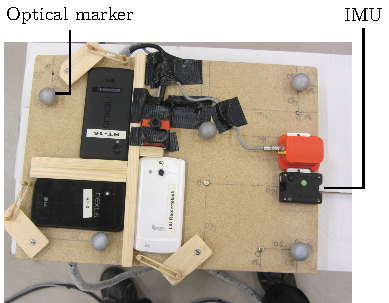
\includegraphics[scale = 1]{figure4_2.pdf}
  \caption{Experimental setup where an \gls{imu} is used to collected inertial and magnetometer measurements. Optical markers are tracked using multiple cameras, leading to accurate reference position and orientation estimates. Note that the experimental setup also contains additional \glspl{imu} and smartphones. The data from these sensors is not considered in this work.}
  \label{fig:oriEst-expSetup}
\end{figure}

\begin{figure}
	\centering
	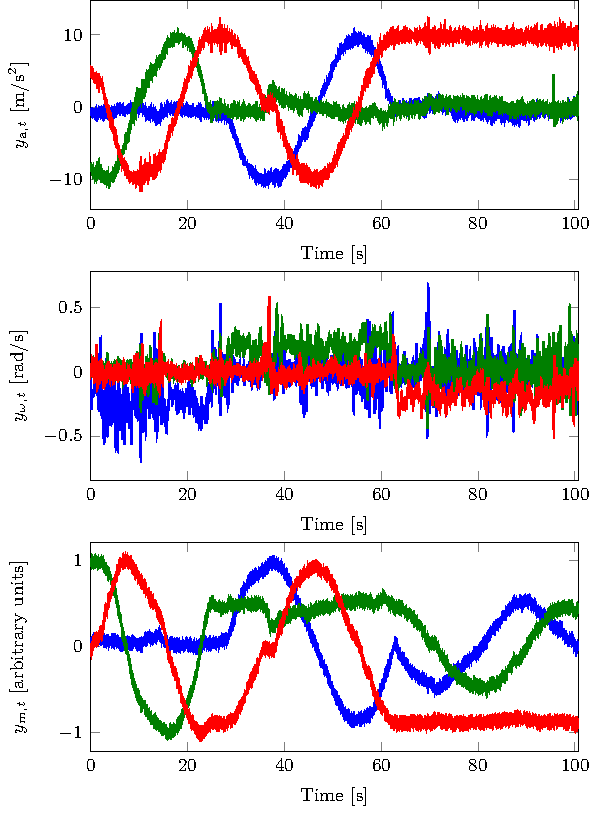
\includegraphics[scale = 1]{figure4_3.pdf}
    	\caption{Measurements from an accelerometer ($y_{\text{a},t}$, top), a gyroscope ($y_{\omega,t}$, middle) and a magnetometer ($y_{\text{m},t}$, bottom) for $100$ seconds of data collected with the \gls{imu} shown in \Figureref{fig:oriEst-expSetup}.}
	\label{fig:oriEst-expDataViconLab}
\end{figure}

\begin{figure}
	\centering
	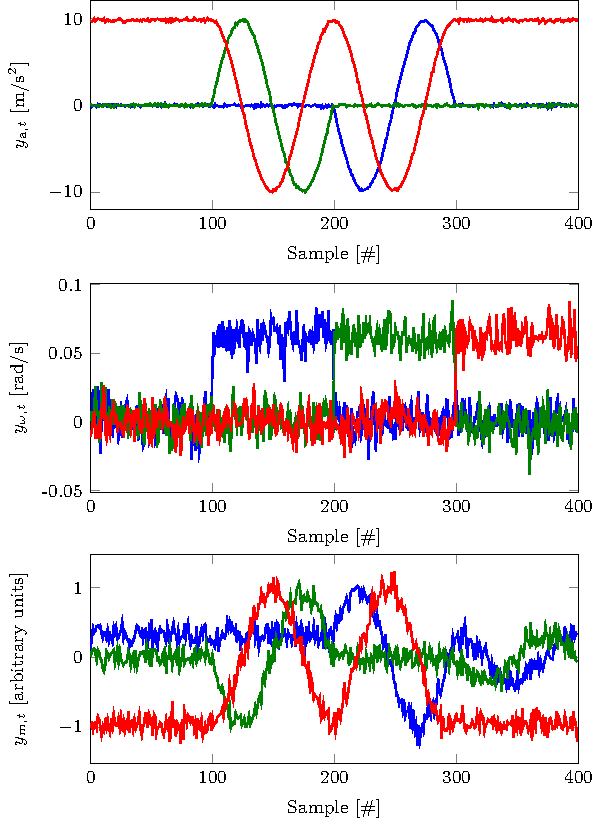
\includegraphics[scale = 1]{figure4_4.pdf}
    	\caption{Simulated measurements from an accelerometer ($y_{\text{a},t}$, top), a gyroscope ($y_{\omega,t}$, middle) and a magnetometer ($y_{\text{m},t}$, bottom).}
	\label{fig:oriEst-simData}	
\end{figure}

In \Figureref{fig:oriEst-simData}, simulated inertial and magnetometer measurements are displayed. The data represents a sensor that is kept stationary for 100 samples, after which it is rotated around all three axes. The sensor is assumed to be rotated around the origin of the accelerometer triad. Hence, during the entire data set, the accelerometer is assumed to only measure the gravity vector. The magnitude of the simulated gravity vector is $9.82~\metrepersquaresecond$. The magnitude of the simulated local magnetic field is equal to one. Its direction is approximately equal to that in Link\"oping, Sweden, where a dip angle of $71^\circ$ leads to a magnetic field  $m^\text{n} = \begin{pmatrix} 0.33 & 0 & - 0.95 \end{pmatrix}^\Transp$. The simulated noise levels are
\begin{align*}
e_{\text{a},t} &\sim \mathcal{N}(0, \sigma_\text{a}^2 \, \mathcal{I}_3), \qquad & \sigma_\text{a} &= 1 \cdot 10^{-1}, \\
e_{\omega,t} &\sim \mathcal{N}(0, \sigma_\omega^2 \, \mathcal{I}_3), \qquad & \sigma_\omega &= 1 \cdot 10^{-2}, \\
e_{\text{m},t} &\sim \mathcal{N}(0, \sigma_\text{m}^2 \, \mathcal{I}_3), \qquad & \sigma_\text{m} &= 1 \cdot 10^{-1}. 
\end{align*}
Note that we deliberately chose the noise levels to be fairly high, to clearly illustrate the workings of the different algorithms. 

Although our algorithms parametrize the orientation as quaternions, it is typically more intuitive to visualize the orientation estimates in Euler angles. Hence, we visualize our results in terms of roll, pitch and heading (yaw) angles. Both for the experimental data and for the simulated data, we are able to compare our estimates $\hat{q}^{\text{nb}}_t$ to reference orientations denoted $q^{\text{nb}}_{\text{ref},t}$. To represent the orientation error, we compute a difference quaternion $\Delta q_t$ as
\begin{align}
\Delta q_t = \hat{q}^{\text{nb}}_t \odot \left( q_{\text{ref},t}^\text{nb} \right)^\conj,
\end{align}
which can be converted to Euler angles for visualization. Note that using this definition, the orientation errors in Euler angles can be interpreted as the errors in roll, pitch and heading.

\subsection{General characteristics}
In this section, we will discuss some general characteristics of the orientation estimation problem and illustrate them in three different examples. Our goal is not to compare the different estimation algorithms, but to illustrate some characteristics common to all of them. 

In \Exampleref{ex:oriEst-simOriErrors} we focus on the accuracy of the orientation estimates that can be obtained if the state space model~\eqref{eq:models-ssOri} is completely true. We illustrate that it is typically easier to obtain accurate roll and pitch estimates than it is to obtain accurate heading estimates. 

\begin{myexample}{Orientation estimation using inertial and magnetometer data}%
\label{ex:oriEst-simOriErrors}%
The orientation errors from the smoothing optimization approach in \Algorithmref{alg:oriEst-smoothingOpt} using simulated inertial and magnetometer measurements as illustrated in \Figureref{fig:oriEst-simData} are depicted in the top plot of \Figureref{fig:oriEst-simOriErrors}. For comparison we also show the orientation errors from dead-reckoning the gyroscope measurements in the bottom plot (see also \Sectionref{sec:intro-imusForPose}). These errors can be seen to drift over time. 

Although the accelerometer and the magnetometer measurement noises are of equal magnitude, the heading angle is estimated with less accuracy compared to the roll and pitch angles. The reason for this is twofold. First, the signal to noise ratio for the magnetometer is worse than that of the accelerometer, since the magnetometer signal has a magnitude of $1$ while the accelerometer signal has a magnitude of $9.82~\metrepersquaresecond$. Second, only the horizontal component of the local magnetic field vector provides heading information. This component is fairly small due to the large dip angle ($71^\circ$) in Link\"oping, Sweden. 
\end{myexample}

\begin{figure}[t]
	\centering
	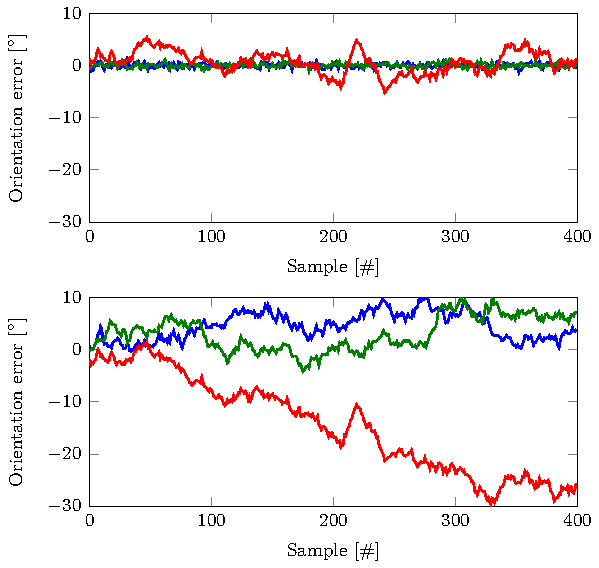
\includegraphics[scale = 1]{figure4_5.pdf}
    	\caption{Orientation errors in roll (blue), pitch (green) and heading (red) using simulated measurements for (top) \Algorithmref{alg:oriEst-smoothingOpt} using inertial and magnetometer measurements and (bottom) dead-reckoning of the gyroscope measurements.}
	\label{fig:oriEst-simOriErrors}
\end{figure}

The accelerometer provides inclination information, while the magnetometer provides heading information, see \Sectionref{sec:models-measModels}. In case only inertial measurements and no magnetometer measurements are available, the heading can only be estimated using the gyroscope measurements and will therefore drift over time. This is illustrated in \Exampleref{ex:oriEst-noMagData}.

\begin{myexample}{Orientation estimation using only inertial measurements}%
\label{ex:oriEst-noMagData}%
The orientation errors from the smoothing optimization approach in \Algorithmref{alg:oriEst-smoothingOpt} using simulated inertial measurements as presented in \Figureref{fig:oriEst-simData} can be found in \Figureref{fig:oriEst-noMagData}. The roll and pitch angles can be seen to be accurate, while the heading angle drifts significantly. To obtain the results in \Figureref{fig:oriEst-noMagData}, we used data with the same noise realization as in \Exampleref{ex:oriEst-simOriErrors}. Hence, we refer to \Figureref{fig:oriEst-simOriErrors} for comparison to the orientation errors from dead-reckoning the gyroscope measurements. The drift in the heading angle can be seen to be similar to the drift from dead-reckoning of the gyroscope measurements. 

\begin{figure}[t]
	\centering
	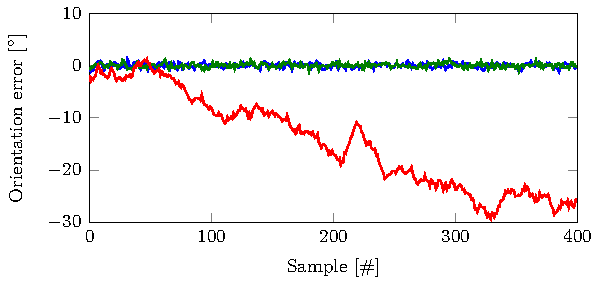
\includegraphics[scale = 1]{figure4_6.pdf}
    	\caption{Orientation errors in roll (blue), pitch (green) and heading (red) using simulated measurements for \Algorithmref{alg:oriEst-smoothingOpt} using inertial measurements only.}
	\label{fig:oriEst-noMagData}
\end{figure}
\end{myexample}

The two examples above assume that our state space model~\eqref{eq:models-ssOri} is an accurate description of the measurements. In practice, however, this is not always the case, for instance due to the presence of magnetic material in the vicinity of the sensor. In \Exampleref{ex:oriEst-magDist} we illustrate that if the state space model does not accurately describe the data, it is not possible to obtain accurate orientation estimates. 

\begin{myexample}{Orientation estimation in the presence of magnetic material}%
\label{ex:oriEst-magDist}%
We simulate 400 samples of stationary data. Between samples 150 and 250, we simulate the presence of a magnetic material, causing a change in the magnetic field of $\begin{pmatrix} 0.1 & 0.3 & 0.5 \end{pmatrix}^\Transp$. In \Figureref{fig:oriEst-magDist}, we show the adapted magnetometer data and the orientation estimates using the smoothing optimization approach from \Sectionref{sec:oriEst-smoothingOpt}. As can be seen, the heading estimates show significant errors when the magnetic material is present. Depending on the amount of disturbance and the uncertainty in the inertial and magnetometer measurements, magnetic material can also result in errors in the roll and pitch estimates. 

\begin{figure}[t]
	\centering
	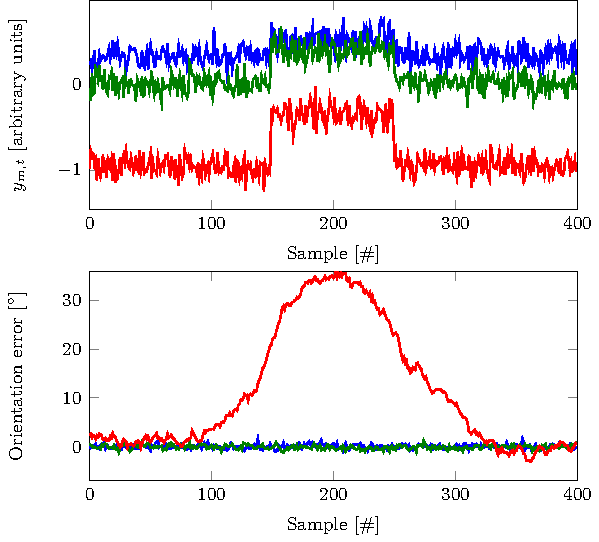
\includegraphics[scale = 1]{figure4_7.pdf}
    	\caption{Top: Simulated magnetometer measurements $y_{\text{m},t}$ for $400$ samples of stationary data. Between samples 150 and 250 we simulate the presence of a magnetic material in the vicinity of the sensor. Bottom: Orientation estimates in roll (blue), pitch (green) and heading (red) using the simulated inertial and magnetometer measurements.}
	\label{fig:oriEst-magDist}
\end{figure}
\end{myexample}

\subsection{Representing uncertainty}
\label{sec:oriEst-repreUncert}
So far, we have discussed the \emph{quality} of the orientation estimates in three different examples. However, we did not discuss the \emph{uncertainty} of the estimates. Algorithms~\ref{alg:oriEst-smoothingOpt}--\ref{alg:oriEst-ekfOriError} provide estimates of the uncertainties. We will now discuss how these uncertainties can be displayed and interpreted and highlight some difficulties with this. 

Both the optimization and the \gls{ekf} approaches discussed in \Sectionref{sec:oriEst-smoothingOpt}--\Sectionref{sec:oriEst-ekf} compute the uncertainty of the estimates in terms of a covariance matrix. Let us use the more general notation $\cov ( \hat{\eta}_t^\text{n})$ for the covariance of the orientation deviation states $\hat{\eta}_t^\text{n}$, $t = 1, \hdots, N$ computed in Algorithms~\ref{alg:oriEst-smoothingOpt},~\ref{alg:oriEst-filteringOpt} and~\ref{alg:oriEst-ekfOriError}, and $\cov ( \hat{q}_t^\text{nb})$ for the covariance of the quaternion states $\hat{q}_t^\text{nb}$, $t = 1, \hdots, N$ computed in \Algorithmref{alg:oriEst-ekfQuat}. If the states would be in normal, Euclidean space, the square root of the diagonal of these matrices would represent the standard deviation $\sigma$ of the estimates in the different directions. These could then be visualized by for instance plotting $3 \sigma$ confidence bounds around the estimates. 

One could imagine that an equivalent way of visualizing the orientation deviation uncertainties, would be to compute the $3 \sigma$ bounds in terms of orientation deviations in each of the three directions as
\begin{subequations}
\begin{align}
\left( \Delta \oriError_{i,t}^\text{n} \right)_{+3 \sigma} &= + 3 \sqrt{\left( \cov (\hat{\oriError}_t^\text{n} \right)_{ii}}, \quad & i &= 1, \hdots, 3, \\
\left( \Delta \oriError_{i,t}^\text{n} \right)_{-3 \sigma} &= - 3 \sqrt{\left( \cov (\hat{\oriError}_t^\text{n} \right)_{ii}}, \quad & i &= 1, \hdots, 3,
\end{align}
\end{subequations}
after which the bounds can be parametrized in terms of quaternions as
\begin{subequations}
\begin{align}
\left( q_t^\text{nb} \right)_{+3 \sigma} = \expq \left( \Delta \oriError_{t}^\text{n} \right)_{+3 \sigma} \odot \hat{q}_t^\text{nb}, \\
\left( q_t^\text{nb} \right)_{-3 \sigma} = \expq \left( \Delta \oriError_{t}^\text{n} \right)_{-3 \sigma} \odot \hat{q}_t^\text{nb}.
\end{align}
\end{subequations}
The resulting estimates and bounds are visualized in terms of Euler angles in \Figureref{fig:oriEst-eulerAngleBounds} for simulated data similar to the data presented in \Figureref{fig:oriEst-simData}. The orientation and its covariance are estimated using \Algorithmref{alg:oriEst-ekfOriError}. As can be seen, the bounds are difficult to interpret due to the wrapping of the Euler angles. 

\begin{figure}
	\centering
	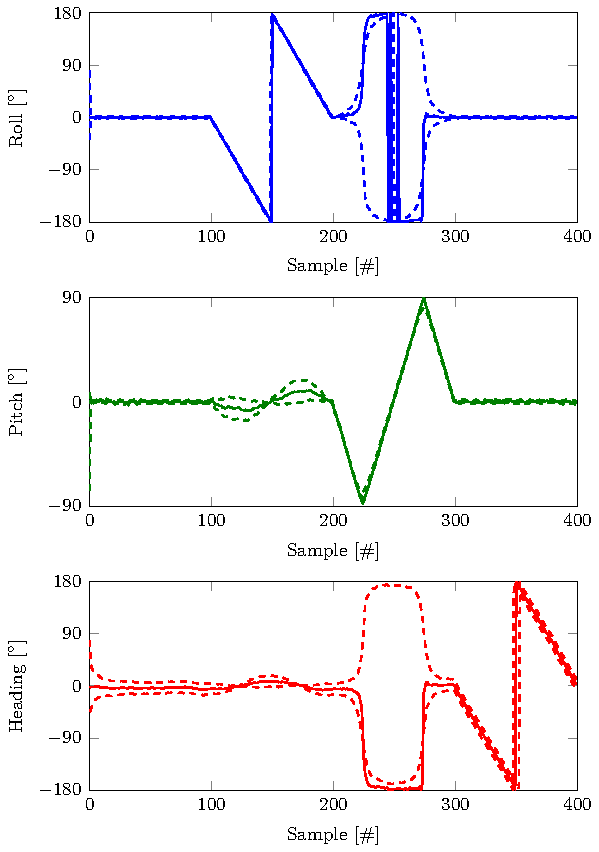
\includegraphics[scale = 1]{figure4_8.pdf}
    	\caption{Orientation estimates (solid) and $3 \sigma$ bounds (dashed) in roll (blue), pitch (green) and heading (red) using inertial and magnetometer measurements.}
	\label{fig:oriEst-eulerAngleBounds}
\end{figure}

As argued in~\cite{forsterCDS:2016}, it is more intuitive to directly represent the uncertainty in terms of orientation deviations. The covariance $\cov ( \hat{\oriError}_t^\text{n})$ can be interpreted as the uncertainty in the roll, pitch and heading angles as illustrated in \Exampleref{ex:oriEst-noMagDataCov}.

\begin{myexample}{Orientation estimation using only inertial measurements (continued)}
\label{ex:oriEst-noMagDataCov}%
Since the accelerometer provides only inclination information, in the case of \Exampleref{ex:oriEst-noMagData} where magnetometer measurements are unavailable, we expect only the roll and pitch angles to be estimated with small uncertainty. In fact, we expect the uncertainty of the heading at $t = 1$ to be equal to the uncertainty of the initial $\Sigma_\text{i}$ from \Sectionref{sec:models-prior} and to steadily grow over time, depending on the amount of gyroscope noise. In \Figureref{fig:oriEst-uncertaintySmoothingNoMag}, we plot the standard deviation $\sigma$ of the orientation estimates computed using the smoothing algorithm from \Sectionref{sec:oriEst-smoothingOpt} as the square root of the diagonal elements of $\cov ( \hat{\eta}_t^\text{n})$. As can be seen, the standard deviation of the yaw angle at $t = 1$ is indeed $20^\circ$ as modeled in \Sectionref{sec:models-prior}. The increase in the uncertainty in the yaw angle exactly matches the increase of the uncertainty due to dead-reckoning. 

\begin{figure}
	\centering
	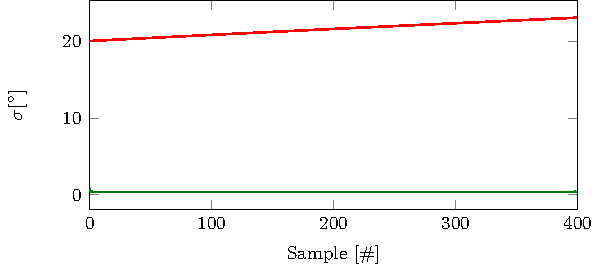
\includegraphics[scale = 1]{figure4_9.pdf}
    	\caption{Standard deviation $\sigma$ in degrees of the orientation estimates in roll (blue), pitch (green) and heading (red) using only inertial measurements.}
	\label{fig:oriEst-uncertaintySmoothingNoMag}
\end{figure}
\end{myexample}

From \Exampleref{ex:oriEst-noMagDataCov} it can be concluded that $\cov ( \hat{\oriError}_t^\text{n})$ seems to be an intuitive measure of the uncertainty of the orientation estimates. The covariance $\cov (\hat{q}_t^\text{nb})$ computed by \Algorithmref{alg:oriEst-ekfQuat} relates to $\cov ( \hat{\oriError}_t^\text{n})$ as
\begin{subequations}
\label{eq:oriEst-convertCovqn}
\begin{align}
\cov (\hat{q}_t^\text{nb}) &= \cov \left(\expq (\tfrac{\hat{\oriError}_t^\text{n}}{2} ) \odot \tilde{q}_t^\text{nb} \right) \nonumber \\
&= \tfrac{1}{4} \left( \tilde{q}_t^\text{nb} \right)^\rightMult \tfrac{\diff \expq(\hat{\oriError}_t^\text{n})}{\diff \hat{\oriError}_t^\text{n}} \cov (\hat{\oriError}_t^\text{n}) \left( \tfrac{\diff \expq(\hat{\oriError}_t^\text{n})}{\diff \hat{\oriError}_t^\text{n}} \right)^\Transp \left( \tilde{q}_t^\text{bn} \right)^\rightMult, \\
\cov (\hat{\oriError}_t^\text{n}) &= \cov \left( 2 \logq ( \hat{q}_t^\text{nb} \odot \tilde{q}_t^\text{bn}  ) \right) \nonumber \\
&= 4 \tfrac{\diff \logq (q)}{\diff q} \left( \tilde{q}_t^\text{bn} \right)^\rightMult \cov ( \hat{q}_t^\text{nb} ) \left( \tilde{q}_t^\text{nb} \right)^\rightMult \left( \tfrac{\diff \logq (q)}{\diff q} \right)^\Transp.
\end{align}
\end{subequations}
The relation~\eqref{eq:oriEst-convertCovqn} allows us to compare the orientation estimates and covariances from the different algorithms in more detail in \Exampleref{ex:oriEst-noMagDataCovComp}. 

\begin{myexample}{Orientation estimation using only inertial measurements (continued)}
\label{ex:oriEst-noMagDataCovComp}
As discussed in \Exampleref{ex:oriEst-noMagDataCov}, using only inertial measurements and no magnetometer measurements, we can only expect to be able to accurately estimate the inclination. The uncertainty of the heading estimates grows over time. We will now analyze the behavior of the different algorithms in more detail for this specific example. In \Tableref{tab:oriEst-rmsNoMagData}, we show the \gls{rmse} values over $100$ Monte Carlo simulations for Algorithms~\ref{alg:oriEst-smoothingOpt}--\ref{alg:oriEst-ekfOriError}. In \Figureref{fig:oriEst-noMagDataEstAll}, we also represent the orientation estimates from the four algorithms for one of these realizations. As can be seen from both \Tableref{tab:oriEst-rmsNoMagData} and \Figureref{fig:oriEst-noMagDataEstAll}, as expected, the smoothing algorithm outperforms the other algorithms. However, more surprisingly, the \gls{ekf} with quaternion states has much larger errors in the heading angle. In \Figureref{fig:oriEst-noMagDataCovAll}, we also show the standard deviations of the estimates from all algorithms. As can be seen, the \gls{ekf} with quaternion states over-estimates its confidence in the estimates of the heading direction. This can most likely be attributed to linearization issues. 

\begin{table}
\caption{Mean \gls{rmse} values over $100$ Monte Carlo simulations estimating orientation using only inertial measurements.}
\label{tab:oriEst-rmsNoMagData}
\begin{center}
\small
\begin{tabular}{lccc}
\toprule
\Gls{rmse} & Roll [$^\circ$]& Pitch [$^\circ$] & Heading [$^\circ$] \\
\midrule
Smoothing optimization (\Algref{alg:oriEst-smoothingOpt}) & 0.39 & 0.39 & 7.46 \\
Filtering optimization (\Algref{alg:oriEst-filteringOpt}) & 0.46 & 0.46 & 7.46 \\
EKF quaternions (\Algref{alg:oriEst-ekfQuat}) & 0.46 & 0.46 & 17.49 \\
EKF orientation deviation (\Algref{alg:oriEst-ekfOriError}) & 0.46 & 0.46 & 7.46 \\
\bottomrule
\end{tabular}
\normalsize
\end{center}
\end{table}

\begin{figure}[t]
	\centering
  	\subfigure[Smoothing optimization (\Algref{alg:oriEst-smoothingOpt}).]{
		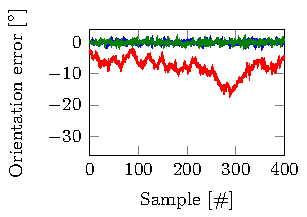
\includegraphics[scale = 1]{figure4_10a.pdf}
		}
	\subfigure[Filtering optimization (\Algref{alg:oriEst-filteringOpt}).]{
		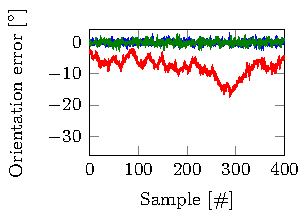
\includegraphics[scale = 1]{figure4_10b.pdf}
		} \\
	\subfigure[EKF quaternions (\Algref{alg:oriEst-ekfQuat})]{
		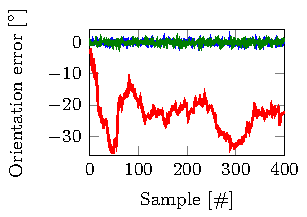
\includegraphics[scale = 1]{figure4_10c.pdf}
		}
	\subfigure[EKF orientation deviation (\Algref{alg:oriEst-ekfOriError}).]{
		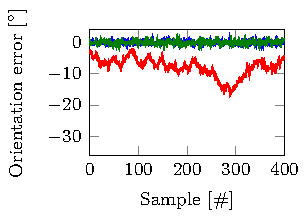
\includegraphics[scale = 1]{figure4_10d.pdf}
		}
  \caption{Orientation estimates of Algorithms~\ref{alg:oriEst-smoothingOpt}--\ref{alg:oriEst-ekfOriError} in roll (blue), pitch (green) and heading (red) using only inertial measurements.}
  \label{fig:oriEst-noMagDataEstAll}
\end{figure}

\begin{figure}[t]
	\centering
  	\subfigure[Smoothing optimization (\Algref{alg:oriEst-smoothingOpt}).]{
		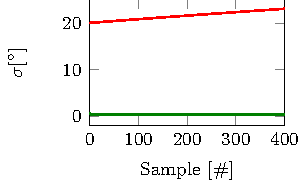
\includegraphics[scale = 1]{figure4_11a.pdf}
		}
	\subfigure[Filtering optimization (\Algref{alg:oriEst-filteringOpt}).]{
		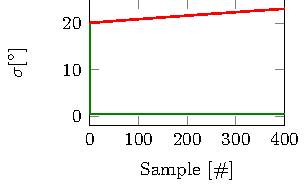
\includegraphics[scale = 1]{figure4_11b.pdf}
		} \\
	\subfigure[EKF quaternions (\Algref{alg:oriEst-ekfQuat}).]{
		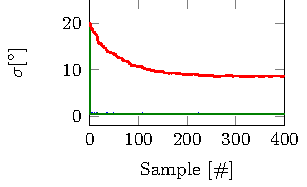
\includegraphics[scale = 1]{figure4_11c.pdf}
		}
	\subfigure[EKF orientation deviation (\Algref{alg:oriEst-ekfOriError}).]{
		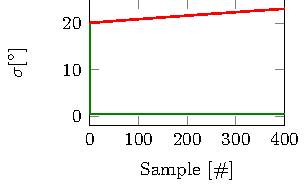
\includegraphics[scale = 1]{figure4_11d.pdf}
		}
  \caption{Standard deviation $\sigma$ in degrees of the orientation estimates of Algorithms~\ref{alg:oriEst-smoothingOpt}--\ref{alg:oriEst-ekfOriError} in roll (blue), pitch (green) and heading (red) using only inertial measurements.}
  \label{fig:oriEst-noMagDataCovAll}
\end{figure}
\end{myexample}

From \Exampleref{ex:oriEst-noMagDataCovComp}, it can be concluded that not properly estimating the covariance can have negative effects on the quality of the estimates. It can also be concluded from this section that covariances can best be represented in terms of $\cov(\hat{\oriError}_t^\text{n})$ but that they are difficult to visualize in Euler angles. Because of that, in the remainder of this section, we will typically plot the uncertainty in a separate plot like in \Figureref{fig:oriEst-noMagDataCovAll}.

\subsection{Comparing the different algorithms}
We use the experimental data presented in \Figureref{fig:oriEst-expDataViconLab} to assess the quality of the estimates from the different algorithms. We also have a short sequence of stationary data available that allows us to determine the gyroscope bias and the sensor noise covariances. The gyroscope bias is subtracted from the data to allow for better orientation estimates. The standard deviation of the gyroscope noise is experimentally determined to be $\sigma_\omega = 4.9 \cdot 10^{-3}$. As discussed in \Sectionref{sec:models-measModels}, the covariance matrices in the measurement models reflect not only the sensor noise, but also the model uncertainty. Both the assumptions that the sensor's acceleration is zero and that the magnetic field is homogeneous are only approximately true. Because of this, we choose $\sigma_\text{a} = 2.6 \cdot 10^{-1}$ and $\sigma_\text{m} = 2.5 \cdot 10^{-1}$. These values are a factor 10 respectively 100 larger than the experimentally determined noise values. Note that this choice is highly dependent on the data set. The \gls{rmse} values as compared to the optical reference system for the different methods described in this chapter are summarized in \Tableref{tab:oriEst-rmsExp}. A good value for $\alpha$ in the complementary filter is experimentally determined to be $0.001$ for this specific data set. As an illustration of the estimates, the orientation estimates as obtained using the smoothing algorithm and the orientations from the optical reference system are shown in \Figureref{fig:oriEst-oriExpResults}. 

It is of course difficult to draw quantitative conclusions based on only one data set. The \gls{rmse} values in \Tableref{tab:oriEst-rmsExp} should therefore mainly be seen as an indication of the performance. Comparing the different algorithms amongst each other is hard. In fact, the algorithms perform differently with respect to each other for different choices of the covariance matrices. Because of this, we will study the accuracy of the different methods using simulated data instead. 

\begin{table}
\caption{RMSE of the orientation estimates obtained using Algorithms~\ref{alg:oriEst-smoothingOpt}--\ref{alg:oriEst-compl} and the experimental data presented in \Figureref{fig:oriEst-expDataViconLab}.}
\label{tab:oriEst-rmsExp}
\begin{center}
\small
\begin{tabular}{lccc}
\toprule
\Gls{rmse} & Roll [$^\circ$]& Pitch [$^\circ$] & Heading [$^\circ$] \\
\midrule
Smoothing optimization (\Algref{alg:oriEst-smoothingOpt}) & 1.03 & 0.48 & 0.81 \\
Filtering optimization (\Algref{alg:oriEst-filteringOpt}) & 1.14 & 0.56 & 1.28 \\
EKF quaternions (\Algref{alg:oriEst-ekfQuat}) & 1.13 & 0.52 & 1.04 \\
EKF orientation deviation (\Algref{alg:oriEst-ekfOriError}) & 1.14 & 0.56 & 1.28 \\
Complementary filter (\Algref{alg:oriEst-compl}) & 0.95 & 0.62 & 1.55 \\
\bottomrule
\end{tabular}
\normalsize
\end{center}
\end{table}

\begin{figure}
	\centering
	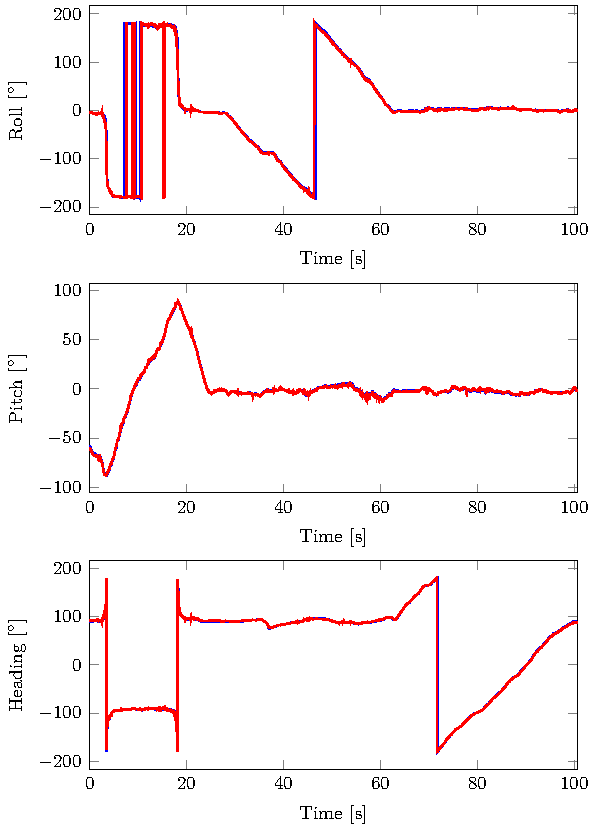
\includegraphics[scale = 1]{figure4_12.pdf}
    	\caption{Red: Orientation from the optical reference system. Blue: Orientation estimates obtained using \Algorithmref{alg:oriEst-smoothingOpt} for the experimental data from \Figureref{fig:oriEst-expDataViconLab}.}
	\label{fig:oriEst-oriExpResults}
\end{figure}

We run 100 Monte Carlo simulations where the simulated data illustrated in \Figureref{fig:oriEst-simData} is generated with different noise realizations.
\Tableref{tab:oriEst-rmsSim} shows the mean \gls{rmse} for the five estimation algorithms. Algorithms~\ref{alg:oriEst-smoothingOpt}--\ref{alg:oriEst-ekfOriError} use the noise covariance matrices that are also used to generate the data. The complementary filter also uses these to determine the orientation from the accelerometer and magnetometer data. To combine this with the orientation from the gyroscope measurements, we need to determine a good value for $\alpha$. We empirically choose a value that leads to good performance for this data set. The orientation from the accelerometer and magnetometer measurements can be expected to be more accurate in the roll and the pitch than in the heading, see \Exampleref{ex:oriEst-simOriErrors}. Since $\alpha$ is scalar, however, it is not possible to weigh these contributions differently. Because of this, we present results both for $\alpha = 0.07$, which leads to small \gls{rmse} values in the heading but relatively larger \gls{rmse} in the roll and the pitch, and for $\alpha = 0.7$, which leads to small \gls{rmse} values in the roll and pitch but large \gls{rmse} in the heading. 

From the results summarized in \Tableref{tab:oriEst-rmsSim}, it can be seen that the smoothing approach outperforms the filtering approaches. The estimates for one of the noise realizations are shown in \Figureref{fig:oriEst-oriSimResultsEstAll}. For Algorithms~\ref{alg:oriEst-smoothingOpt}--\ref{alg:oriEst-ekfOriError}, we also depict the  covariance estimates in \Figureref{fig:oriEst-oriSimResultsCovAll}. The filtering approaches from Algorithms~\ref{alg:oriEst-filteringOpt}--\ref{alg:oriEst-ekfOriError} estimate the standard deviation of the orientation errors at $t = 1$ to be equal to $20^\circ$. After this, they can be seen to converge to around $3.16^\circ$ degrees for the heading angle and $0.46^\circ$ for roll and pitch angles. The smoothing algorithm estimates an uncertainty in the heading angle of around $3.17^\circ$ for the first and last sample, while converging to a standard deviation of $2.25^\circ$ for the middle of the data set. For the roll and pitch angles, the initial and final uncertainties are estimated to be around $0.73^\circ$, converging to $0.39^\circ$ for the middle of the data set. Note that these values correspond fairly well with the \gls{rmse} values in \Tableref{tab:oriEst-rmsSim}. 

\begin{table}[t]
\caption{Mean \gls{rmse} of the orientation estimates from $100$ Monte Carlo simulations using Algorithms~\ref{alg:oriEst-smoothingOpt}--\ref{alg:oriEst-compl}.}
\label{tab:oriEst-rmsSim}
\begin{center}
\small
\begin{tabular}{lccc}
\toprule
\Gls{rmse} & Roll [$^\circ$]& Pitch [$^\circ$] & Heading [$^\circ$] \\
\midrule
Smoothing optimization (\Algref{alg:oriEst-smoothingOpt}) & 0.39 & 0.39 & 2.30 \\
Filtering optimization (\Algref{alg:oriEst-filteringOpt}) &  0.45 & 0.45 & 3.54 \\
EKF quaternions (\Algref{alg:oriEst-ekfQuat}) & 0.45 & 0.45 & 3.57 \\
EKF orientation deviation (\Algref{alg:oriEst-ekfOriError}) & 0.45 & 0.45 & 3.55 \\
Complementary filter (\Algref{alg:oriEst-compl}), $\alpha = 0.07$ & 1.44 & 1.43 & 4.39 \\
Complementary filter (\Algref{alg:oriEst-compl}), $\alpha = 0.7$ & 0.47 & 0.47 & 12.98 \\
\bottomrule
\end{tabular}
\normalsize
\end{center}
\end{table}

\begin{figure}
	\centering
  	\subfigure[Smoothing optimization (\Algref{alg:oriEst-smoothingOpt}).]{
		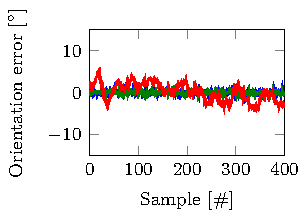
\includegraphics[scale = 1]{figure4_13a.pdf}
		}
	\subfigure[Filtering optimization (\Algref{alg:oriEst-filteringOpt}).]{
		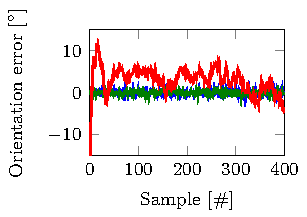
\includegraphics[scale = 1]{figure4_13b.pdf}
		} \\
	\subfigure[EKF quaternions (\Algref{alg:oriEst-ekfQuat}).]{
		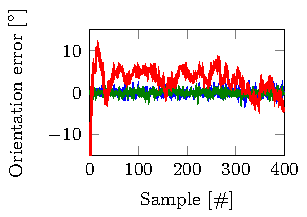
\includegraphics[scale = 1]{figure4_13c.pdf}
		}
	\subfigure[EKF orientation deviation (\Algref{alg:oriEst-ekfOriError}).]{
		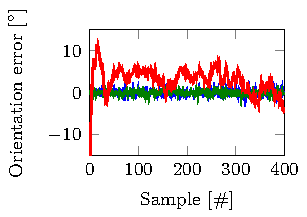
\includegraphics[scale = 1]{figure4_13d.pdf}
		}
	\subfigure[Complementary filter (\Algref{alg:oriEst-compl}), $\alpha = 0.07$.]{
		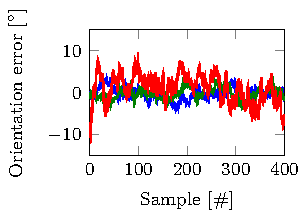
\includegraphics[scale = 1]{figure4_13e.pdf}
		}
	\subfigure[Complementary filter (\Algref{alg:oriEst-compl}), $\alpha = 0.7$.]{
		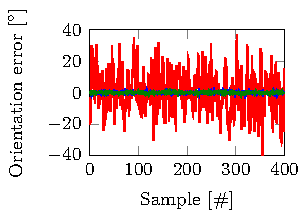
\includegraphics[scale = 1]{figure4_13f.pdf}
		}		
  \caption{Orientation errors of Algorithms~\ref{alg:oriEst-smoothingOpt}--\ref{alg:oriEst-compl} in roll (blue), pitch (green) and heading (red) using simulated inertial and magnetometer measurements.}
  \label{fig:oriEst-oriSimResultsEstAll}
\end{figure}

\begin{figure}[t]
	\centering
  	\subfigure[Smoothing optimization (\Algref{alg:oriEst-smoothingOpt}).]{
		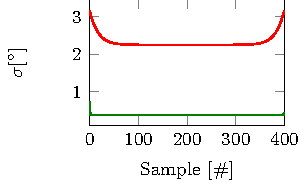
\includegraphics[scale = 1]{figure4_14a.pdf}
		}
	\subfigure[Filtering optimization (\Algref{alg:oriEst-filteringOpt}).]{
		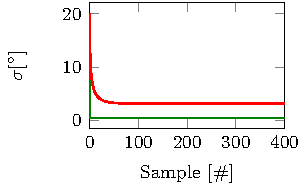
\includegraphics[scale = 1]{figure4_14b.pdf}
		} \\
	\subfigure[EKF quaternions (\Algref{alg:oriEst-ekfQuat}).]{
		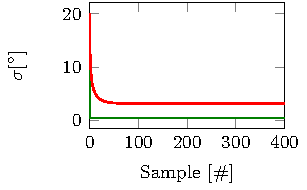
\includegraphics[scale = 1]{figure4_14c.pdf}
		}
	\subfigure[EKF orientation deviation (\Algref{alg:oriEst-ekfOriError}).]{
		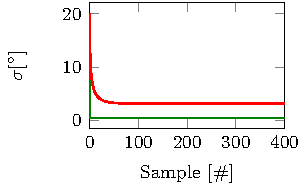
\includegraphics[scale = 1]{figure4_14d.pdf}
		}
  \caption{Standard deviation $\sigma$ in degrees of the orientation estimates of Algorithms~\ref{alg:oriEst-smoothingOpt}--\ref{alg:oriEst-ekfOriError} in roll (blue), pitch (green) and heading (red) using simulated inertial and magnetometer measurements. Note the different scale on the vertical axis of (a) as compared to (b)--(d).}
  \label{fig:oriEst-oriSimResultsCovAll}
\end{figure}

\begin{table}
\caption{Mean \gls{rmse} of the orientation estimates from $100$ Monte Carlo simulations. The estimate of the initial orientation is assumed to be normal distributed around the true initial orientation with a standard deviation of $20^\circ$.}
\label{tab:oriEst-rmsSimWrongInit}
\begin{center}
\small
\begin{tabular}{lccc}
\toprule
\Gls{rmse} & Roll [$^\circ$]& Pitch [$^\circ$] & Heading [$^\circ$] \\
\midrule
Smoothing optimization (\Algref{alg:oriEst-smoothingOpt}) & 0.39 & 0.39 & 2.29 \\
Filtering optimization (\Algref{alg:oriEst-filteringOpt}) &  1.06 & 0.95 & 3.55 \\
EKF quaternions (\Algref{alg:oriEst-ekfQuat}) & 1.08 & 0.97 & 4.41 \\
EKF orientation deviation (\Algref{alg:oriEst-ekfOriError}) & 1.08 & 0.96 & 3.57 \\
Complementary filter (\Algref{alg:oriEst-compl}), $\alpha = 0.07$ & 3.02 & 2.77 & 4.48 \\
Complementary filter (\Algref{alg:oriEst-compl}), $\alpha = 0.7$ & 1.13 & 1.01 & 12.99 \\
\bottomrule
\end{tabular}
\normalsize
\end{center}
\end{table}

For the Monte Carlo simulations described above, the three filtering algorithms perform similarly. However, differences can be seen when an update of the filter needs to correct the orientation estimates significantly. Examples for when this happens are when the initial orientation is not accurately known or when magnetometer measurements are not available for a longer period of time. In these cases, the uncertainty of the state is large and large corrections to the state estimates are needed when measurements become available. To analyze this case in more detail, we assume that the estimate of the initial orientation $\initEst{q}_1^\text{nb}$ is normal distributed around the true initial orientation with a standard deviation of $20^\circ$. Hence, we do not use the first accelerometer and magnetometer data for initialization. Note that a standard deviation of $20^\circ$ is equal to the uncertainty on the initial state assumed by the algorithms. The results for $100$ Monte Carlo simulations are summarized in \Tableref{tab:oriEst-rmsSimWrongInit}. As can be seen, specifically the \gls{ekf} with quaternion states and the complementary filter with $\alpha = 0.07$ perform worse than \Algorithmref{alg:oriEst-filteringOpt} and \Algorithmref{alg:oriEst-ekfOriError} for this data.

Which algorithm to use is highly application-specific. However, in general it can be concluded that all five algorithms actually produce fairly good orientation estimates, assuming that the models from \Sectionref{sec:models-resultingProbModel} are indeed valid. The smoothing algorithm performs better than the filtering approaches but it is also the most computationally expensive. The \gls{ekf} with quaternion states and the complementary filter suffer from linearization issues when large orientation corrections need to be made or when magnetometer data is unavailable.

\section{Extending to pose estimation}
\label{sec:oriEst-poseEstimation}
In \Sectionref{sec:oriEst-orientationEstimation}, we have evaluated the performance of Algorithms~\ref{alg:oriEst-smoothingOpt}--\ref{alg:oriEst-compl} for orientation estimation. The estimation methods presented in \Sectionref{sec:oriEst-smoothingOpt}--\Sectionref{sec:oriEst-ekf} can also be used to estimate the sensor's pose using the state space model~\eqref{eq:models-ssPose}. Complementary filtering is predominantly used for orientation estimation and will therefore not be considered in this section. 

The pose estimation problem can be written as a smoothing optimization problem as 
\begin{align}
\label{eq:oriEst-posSmoothing}
\hat{x}_{1:N} = \argmin_{x_{1:N}} &\underbrace{\vphantom{\sum_{t = 2}^N} \| e_{\text{p,i}} \|_{\Sigma_{\text{p,i}}^{-1}}^2 + \| e_{\text{v,i}} \|_{\Sigma_{\text{v,i}}^{-1}}^2 + \| e_{\oriError,\text{i}} \|_{\Sigma_{\oriError,\text{i}}^{-1}}^2}_{\text{Prior}} + \underbrace{\sum_{t = 2}^N \| e_{\text{p},t} \|_{\Sigma_\text{p}^{-1}}^2}_{\text{Measurement model}} + \nonumber \\
& \quad \underbrace{\sum_{t = 2}^N \| e_{\omega,t} \|_{\Sigma_\omega^{-1}}^2 + \| e_{\text{a,p},t} \|_{\Sigma_\text{a,p}^{-1}}^2 + \| e_{\text{a,v},t} \|_{\Sigma_\text{a,v}^{-1}}^2}_{\text{Dynamics}},
\end{align}
with $x_t = \begin{pmatrix} p_t^\Transp & v_t^\Transp & (\oriError_t^\text{n})^\Transp \end{pmatrix}^\Transp$ and
\begin{subequations}
\label{eq:oriEst-poseSmoothingTerms}
\begin{align}
e_\text{p,i} &= p_1^\text{n} - y_{\text{p},1}, \quad & e_{\text{p,i}} &\sim \mathcal{N}(0,\Sigma_\text{p,i}), \\
e_\text{v,i} &= v_1, \quad & e_{\text{v,i}} &\sim \mathcal{N}(0,\Sigma_\text{v,i}), \\
e_{\oriError,\text{i}} &=  2 \logq \left( q_1^\text{nb} \odot \initEst{q}_1^\text{bn} \right), \quad & e_{\text{i}} &\sim \mathcal{N}(0,\Sigma_{\oriError,\text{i}}), \\
e_{\text{p,a},t} &= \tfrac{2}{T^2} \left( p_{t+1}^\text{n} - p_t^\text{n} - T v_t^\text{n} \right) - & &\nonumber \\
 & \qquad R^\text{nb}_t y_{\text{a},t} -  g^\text{n}, \quad & e_{\text{p,a},t} &\sim \mathcal{N}(0,\Sigma_\text{a}), \label{eq:oriEst-poseSmoothingTerms-posDyn} \\
e_{\text{v,a},t} &= \tfrac{1}{T} \left( v_{t+1}^\text{n} - v_t^\text{n} \right) - R^\text{nb}_t y_{\text{a},t} -  g^\text{n}, \quad & e_{\text{v,a},t} &\sim \mathcal{N}(0,\Sigma_\text{a}), \label{eq:oriEst-poseSmoothingTerms-velDyn} \\
e_{\omega,t} &= \tfrac{2}{T} \logq \left( q_t^\text{bn} \odot q^\text{nb}_{t+1}\right) - y_{\omega,t}, \quad & e_{\omega,t} &\sim \mathcal{N}(0,\Sigma_\omega),  \\
e_{\text{p},t} &= y_{\text{p},t} - p^\text{n}_t, \quad & e_{\text{p},t} &\sim \mathcal{N}(0,\Sigma_\text{p}). 
\end{align}
\end{subequations}
In this section, we will discuss some details about the workings of the pose estimation algorithm using this model. We will not go through a complete derivation of the four algorithms. However, the adaptations that are needed to use Algorithms~\ref{alg:oriEst-smoothingOpt}--\ref{alg:oriEst-ekfOriError} for pose estimation can be found in \Appendixref{app:poseEst}. 

An important observation is that $e_{\text{a,p},t}$ and $e_{\text{a,v},t}$ in \eqref{eq:oriEst-poseSmoothingTerms-posDyn} and \eqref{eq:oriEst-poseSmoothingTerms-velDyn} depend on the orientation $R_t^\text{nb}$. Because of this, the position, velocity and orientation states are coupled. The position measurements therefore do not only provide information about the position and velocity, but also about the orientation of the sensor. This is the reason why it is no longer essential to include magnetometer data and to assume that the acceleration is approximately zero. However, the accuracy of the orientation estimates depends on the movements of the sensor. This will be illustrated below. For this, we simulate 400 samples of inertial and position measurements for a non-rotating sensor with noise levels
\begin{align*}
e_{\text{a},t} &\sim \mathcal{N}(0, \sigma_\text{a}^2 \, \mathcal{I}_3), \qquad & \sigma_\text{a} &= 1 \cdot 10^{-1}, \\
e_{\omega,t} &\sim \mathcal{N}(0, \sigma_\omega^2 \, \mathcal{I}_3), \qquad & \sigma_\omega &= 1 \cdot 10^{-2}, \\
e_{\text{p},t} &\sim \mathcal{N}(0, \sigma_\text{p}^2 \, \mathcal{I}_3), \qquad & \sigma_\text{p} &= 1 \cdot 10^{-2}.
\end{align*}
We consider four different sensor motions. The results in this section are based on the solution to the smoothing optimization problem~\eqref{eq:oriEst-posSmoothing}. First, we simulate data assuming that the sensor is stationary. For this case, the position measurements provide information about the inclination of the sensor, but not about its heading. This is illustrated in \Exampleref{ex:oriEst-poseOriError-stat}.

\begin{myexample}{Pose estimation for a stationary sensor}%
\label{ex:oriEst-poseOriError-stat}%
We estimate the pose of a stationary sensor using simulated data and a smoothing algorithm that solves~\eqref{eq:oriEst-posSmoothing} as described in \Sectionref{sec:oriEst-smoothingOpt}. The orientation error for a specific noise realization is depicted in \Figureref{fig:oriEst-poseOriError-stat}. The inclination errors can be seen to be small, while the heading estimates drift. 
\end{myexample}

\begin{figure}[t]
	\centering
  	\subfigure[Stationary.]{
		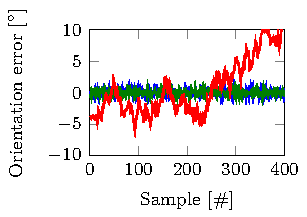
\includegraphics[scale = 1]{figure4_15a.pdf}
		\label{fig:oriEst-poseOriError-stat}
		}
	\subfigure[Constant acceleration.]{
		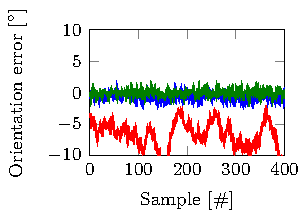
\includegraphics[scale = 1]{figure4_15b.pdf}
		\label{fig:oriEst-poseOriError-const}
		}
		\\
	\subfigure[Acceleration $\left( y_{\text{a},t} \right)_y \sim \mathcal{N}(0,0.5)$.]{
		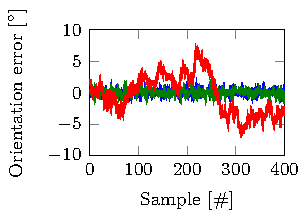
\includegraphics[scale = 1]{figure4_15c.pdf}
		\label{fig:oriEst-poseOriError-rand05}
		}
	\subfigure[Acceleration $\left( y_{\text{a},t} \right)_y \sim \mathcal{N}(0,5)$.]{
		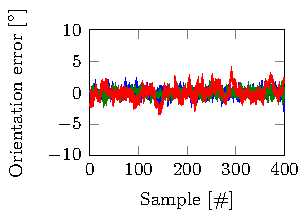
\includegraphics[scale = 1]{figure4_15d.pdf}
		\label{fig:oriEst-poseOriError-rand5}
		\tikzexternalenable 
		}
  \caption{Orientation errors of the roll (blue), pitch (green) and heading (red) using simulated inertial and magnetometer measurements.}
  \label{fig:oriEst-poseOriError}
\end{figure}

Next, in \Exampleref{ex:oriEst-poseOriError-const}, we consider the case where the sensor has a constant linear acceleration. For this case, a drift in the orientation estimates can be seen in the direction that is orthogonal to the direction of the accelerometer measurements.

\begin{myexample}{Pose estimation for a sensor with constant linear acceleration}
\label{ex:oriEst-poseOriError-const}
We estimate the pose of a sensor with an acceleration of $1~\metrepersquaresecond$ in the $y$-direction using simulated data and obtain smoothed estimates by solving~\eqref{eq:oriEst-posSmoothing}. The orientation error for a specific noise realization is depicted in \Figureref{fig:oriEst-poseOriError-const}. Again, a drift can be seen in the orientation estimates. This drift is no longer only in the heading direction, but there is also a small drift on the roll angle.  
\end{myexample}

Finally, in \Exampleref{ex:oriEst-poseOriError-rand} we consider the case of a time-varying linear acceleration. Based on simulated data, we show that accurate heading estimates can be obtained for this case. Furthermore, we show that the larger the acceleration, the more accurate the heading estimates will be. 

\begin{myexample}{Pose estimation for a sensor with time-varying linear acceleration}
\label{ex:oriEst-poseOriError-rand}
We estimate the pose of a sensor with an acceleration in the $y$-direction of $\left( y_{\text{a},t} \right)_y \sim \mathcal{N}(0,0.5)~\metrepersquaresecond$ using simulated data and compute smoothed estimates by solving~\eqref{eq:oriEst-posSmoothing}. The orientation error for a specific noise realization is depicted in \Figureref{fig:oriEst-poseOriError-rand05}. Furthermore, we simulate data with $\left( y_{\text{a},t} \right)_y \sim \mathcal{N}(0,5)~\metrepersquaresecond$. The orientation errors based on this data can be found in \Figureref{fig:oriEst-poseOriError-rand5}. As can be seen, for these cases, it is possible obtain reliable heading estimates using the state space model~\eqref{eq:models-ssPose}. The larger the acceleration, the more accurate the heading estimates.
\end{myexample}

In general, it can be concluded that it is possible to estimate position and orientation using the state space model~\eqref{eq:models-ssPose}. Except in the cases of constant or zero acceleration, it is possible to obtain drift-free orientation estimates. The heading accuracy depends on the amount of acceleration. This is summarized in \Tableref{tab:oriEst-poseOriError} where the mean \gls{rmse} of the state estimates over 100 Monte Carlo simulations is shown. Four cases were considered, inspired by Examples~\ref{ex:oriEst-poseOriError-stat}--\ref{ex:oriEst-poseOriError-rand}.

\begin{table}
\caption{Mean \gls{rmse} of the position and orientation estimates from $100$ Monte Carlo simulations. Considered are a stationary sensor, a sensor with constant acceleration and two cases of time-varying accelerations with different magnitudes.}
\label{tab:oriEst-poseOriError}
\begin{center}
\small
\begin{tabular}{lcccc}
\toprule
\Gls{rmse} & Roll [$^\circ$] & Pitch [$^\circ$] & Heading [$^\circ$] & Position [\centi\meter]\\
\midrule
Stationary & 0.41 & 0.41 & 11.84 & 0.97 \\
Constant acceleration & 1.23 & 0.46 & 11.37 & 0.97 \\ 
Acceleration & \multirow{2}{*}{0.41} & \multirow{2}{*}{0.41} & \multirow{2}{*}{2.68} & \multirow{2}{*}{0.97} \\ 
$\left( y_{\text{a},t} \right)_y \sim \mathcal{N}(0,0.5)$ & & & & \\
Acceleration & \multirow{2}{*}{0.46} & \multirow{2}{*}{0.39} & \multirow{2}{*}{0.87} & \multirow{2}{*}{0.97}  \\ 
$\left( y_{\text{a},t} \right)_y \sim \mathcal{N}(0,5)$ & & & & \\
\bottomrule
\end{tabular}
\normalsize
\end{center}
\end{table}